%!TEX root = ../../thesis.tex
%\subsection{Preliminaries on Lie groups}
\section{Generalized models for soft manipulators} \label{sec:chap3_model}
In this chapter, we will explore Lie group theory applied to deformable robots. We have introduced some of notations earlier in Chapter \ref{chap:PCC}, but for convenience, we briefly recapulate this here. The Lie group of rigid-body transformation on $\R^3$ is denoted by $\SE{3}$. The group of homogeneous rotation is denoted by $\SO{3}$. The tangent space at the identity of the group is called its \textit{Lie algebra}, and it can be used to describe the evolution of the Lie group. The Lie algebras of $\SE{3}$ and $\SO{3}$ are denoted by $\seg{3}$ and $\sog{3}$, respectively. Lastly, the cross operator (\ie, "$\times$") and hat operator (\ie, "$\wedge$") are used to transform a column vector of $\R^3$ or $\R^6$ into an element of the Lie algebra $\sog{3}$ or $\seg{3}$, respectively. A comprehensive introduction is given in Appendix \ref{app:C3:liegroup} based on the work of Murray et al. \cite{Murray1994}. 

\begin{figure}[!t]
  \vspace{-2mm}
  \centering
 %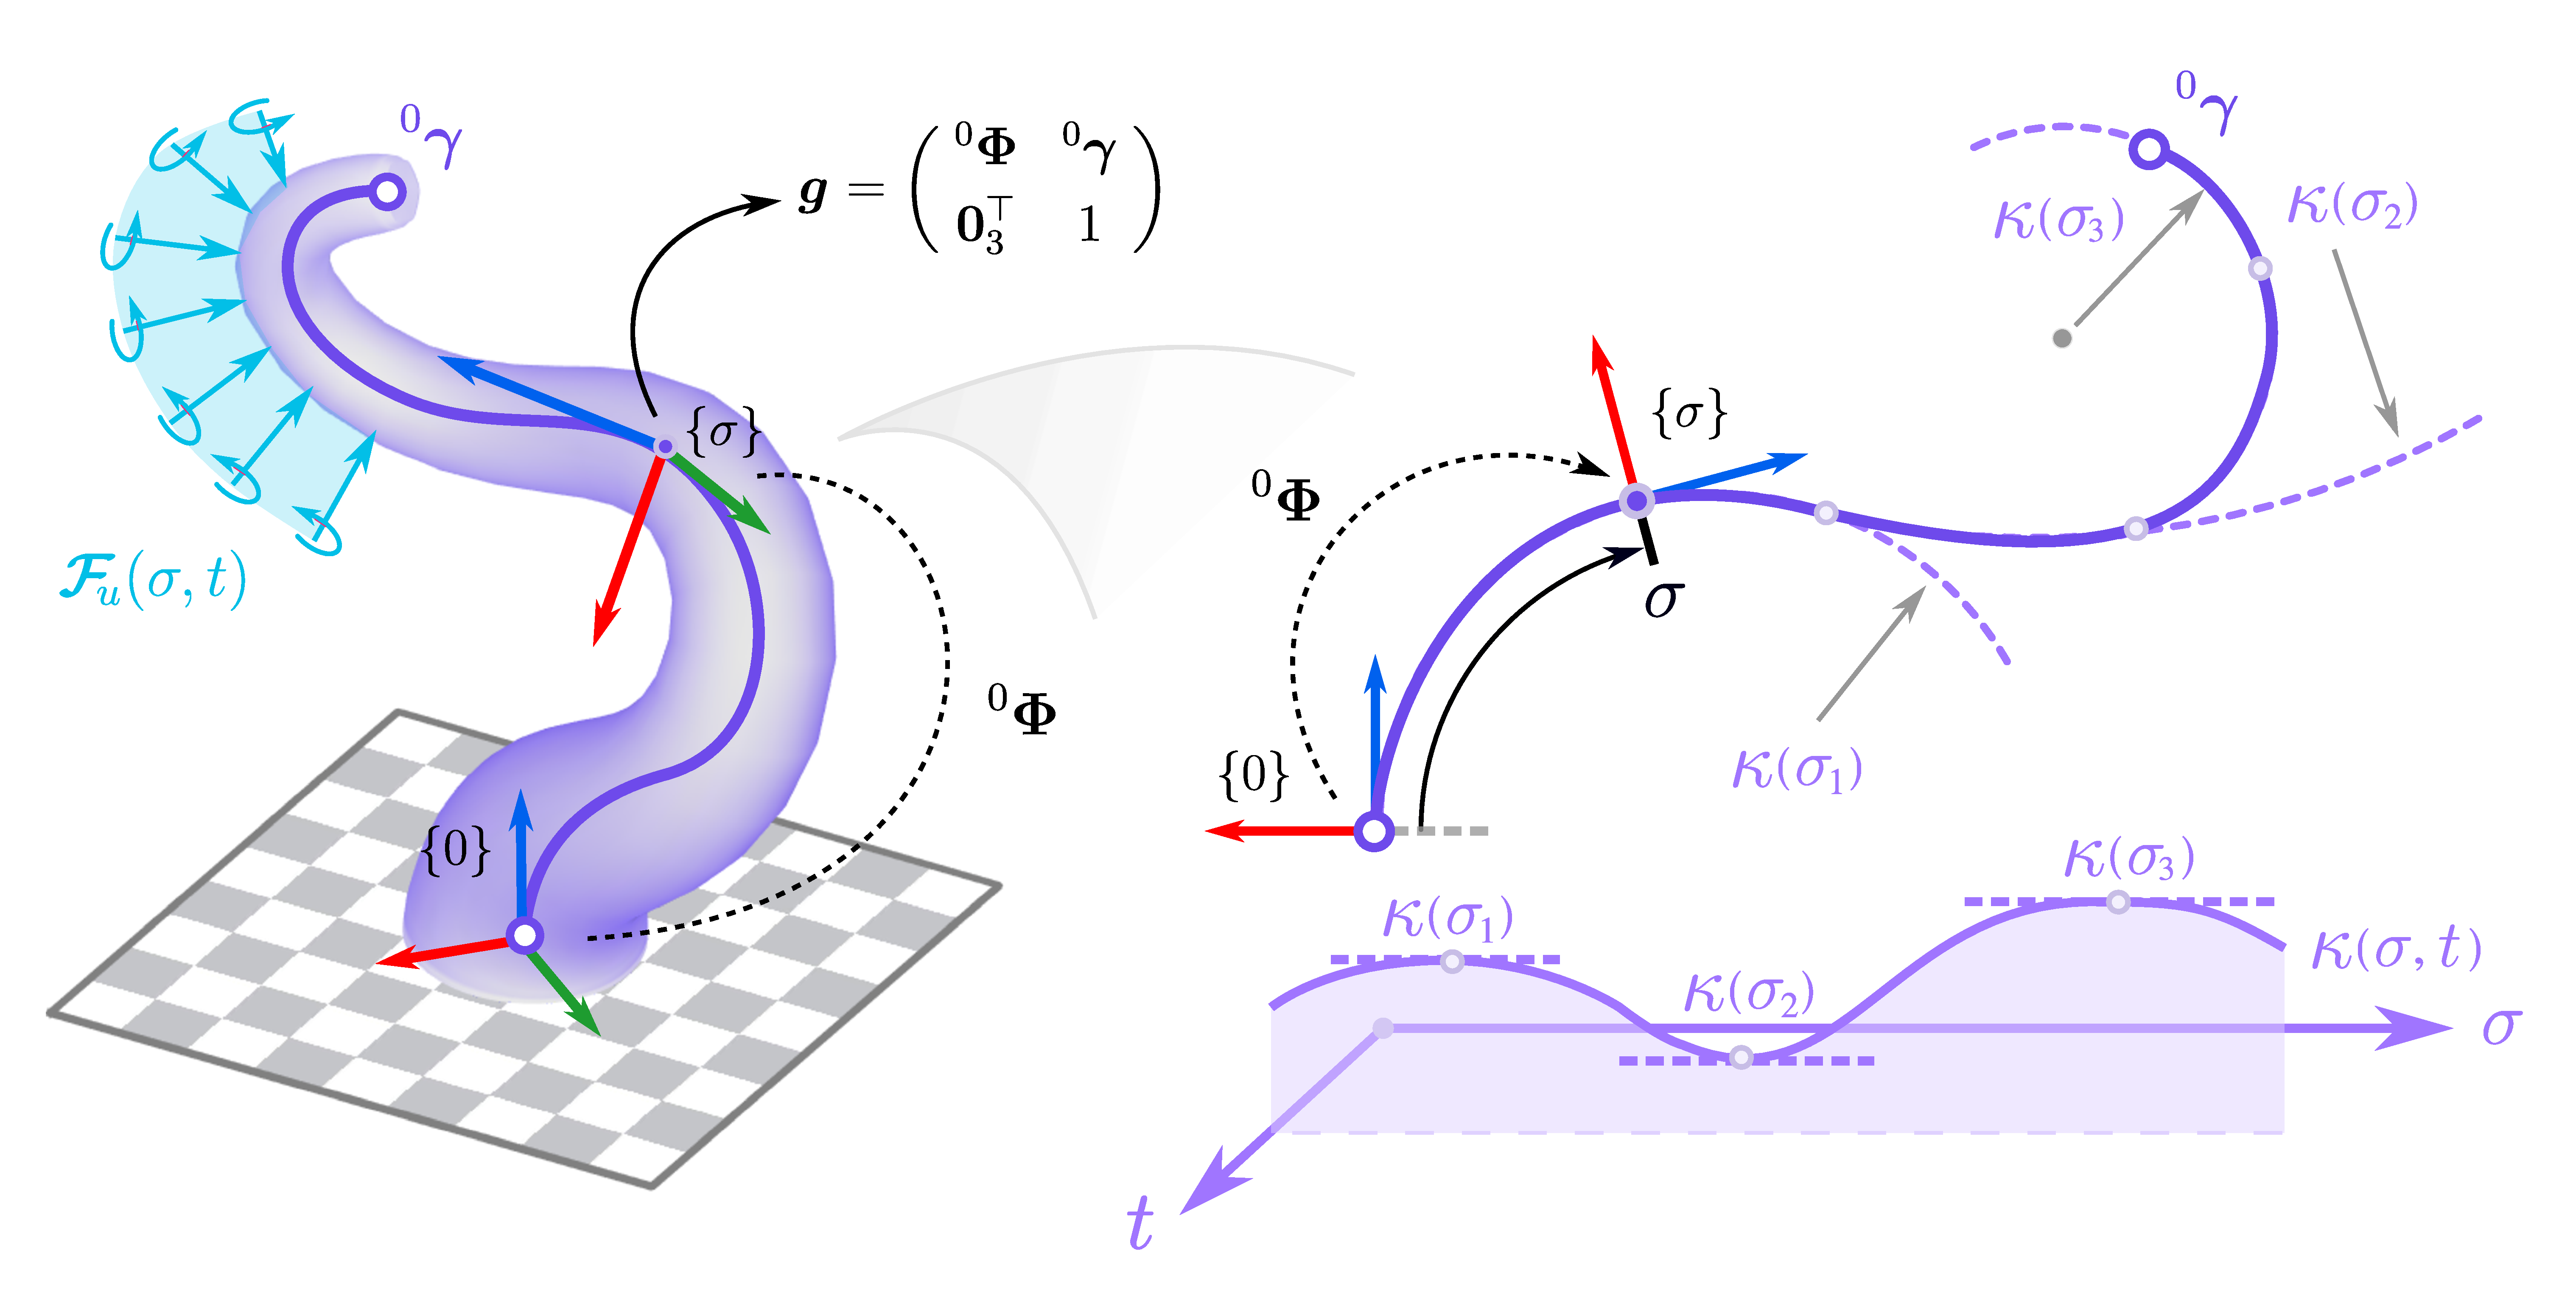
\includegraphics[width = 0.99\textwidth]{3_chapters/3_chapter/img/fig_C3_schematic.pdf}
  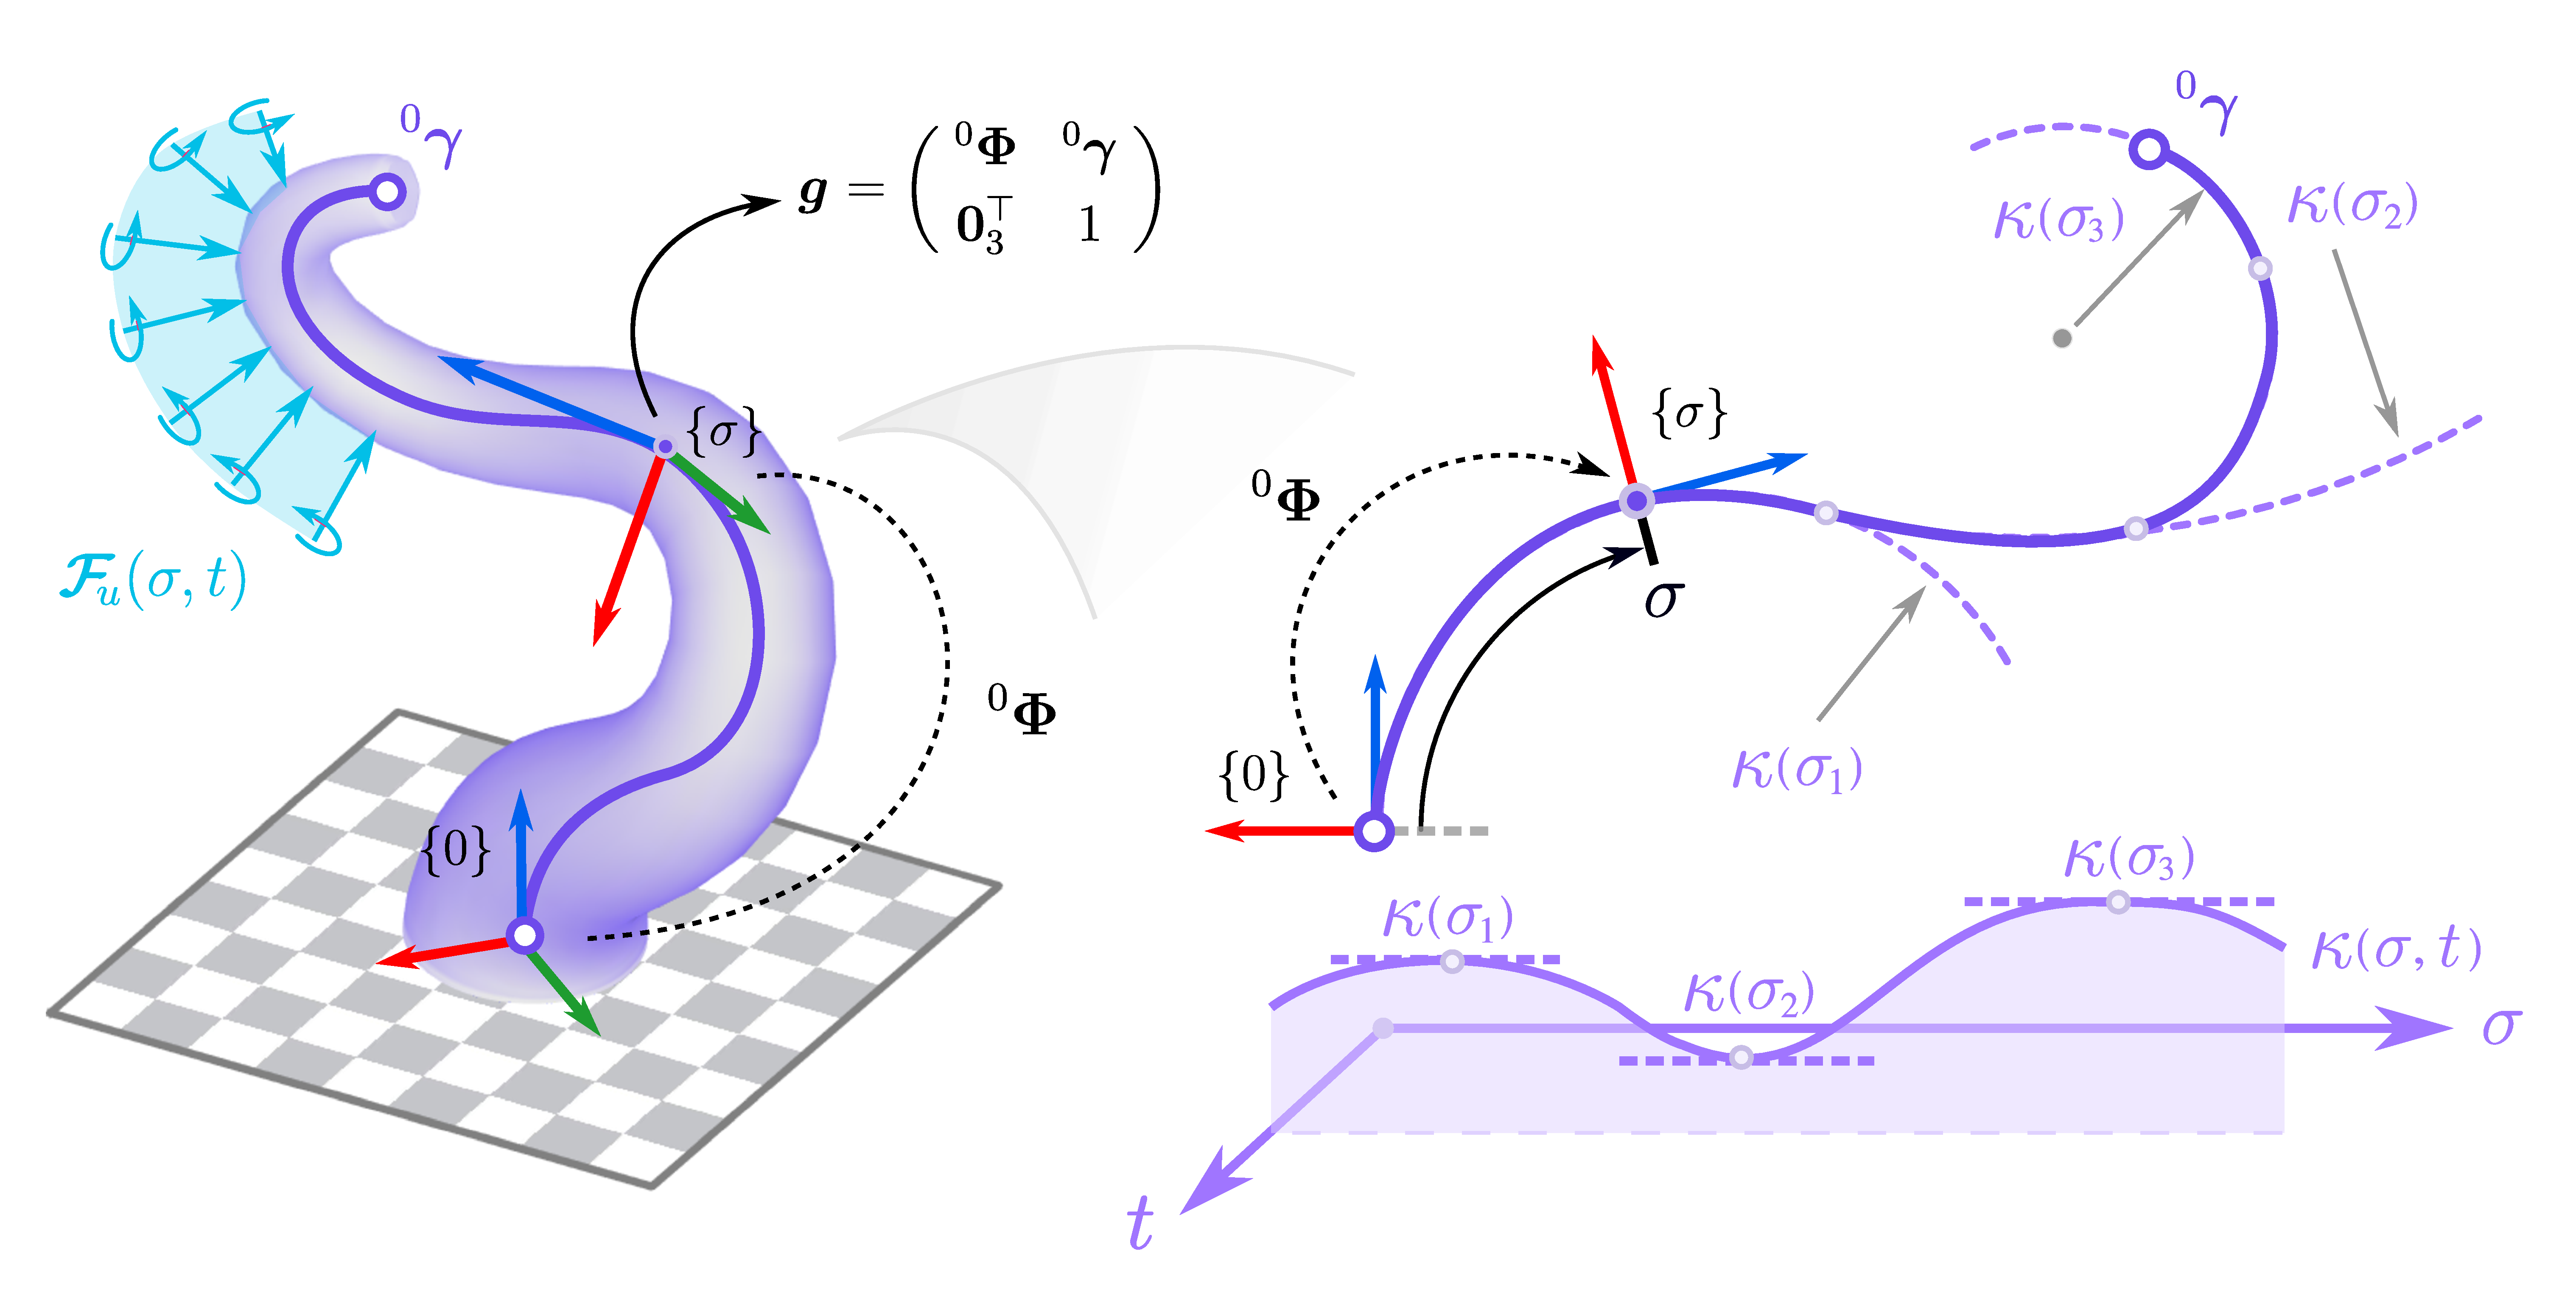
\includegraphics[width = \textwidth]{./pdf/thesis-figure-5-1.pdf}
  \caption{Schematic representation of the continuously variable Cosserat beam model for a general class of soft manipulators, given by a backbone curve $\gammaB$ and orientation matrix $\PhiB$ relative to a base frame at $\{0\}$ Together they form a parameterized curve $\gB(\sigma,t) = (\PhiB(\sigma,t),\, \gammaB(\sigma,t)) \in \SE{3}$. The representation of the soft robot is inspired by the octopus' tentacle whose the muscle forces are modeled as a distributed input $\FT_u$. \label{fig:C3:example1}}
  %\vspace{-0.4cm}
\end{figure}

\subsection{Preliminaries on geometric Cosserat theory}
In Cosserat theory, slender deformable solids are modeled as elastic strings subjected to geometric finite-strain theory. Drawing the analogy to soft robotics, we model the soft robot as a one-dimensional spatial curve passing through the geometric center of the soft robot (see Figure \ref{fig:C3:example1}). Given its spatial-temporal nature, we introduce a temporal variable $t \in [0,+\infty)$, and a spatial variable $\sigma \in [0,\,L]$ with $L$ the undeformed length of the soft robot. For each point on the backbone, we introduce a (mobile) coordinate frame. The homogeneous rotation related to these coordinate frames is given by the rotation matrix $\mat{\Phi}: [0,L] \times [0,+\infty) \to  \SO{3}$, and their origin by the position vector $\vec{\gamma}: [0,L] \times [0,+\infty) \to \R^3$. For convenience and readability, we will denote the temporal and spatial domains as $\Ts = [0,+\infty)$ and $\Xs = [0,\,L]$, respectively.

Following the geometric approach \cite{Simo1986,Boyer2010,Boyer2021,Renda2018,Renda2020}, we may equivalently represent each coordinate frames that are rigidly attached to the continuous backbone of the soft robot by a parameterized space curve in $\SE{3}$:
%
\begin{equation}
\mat{g}(\sigma,t) = \begin{pmatrix} \mat{\Phi}(\sigma,t) & \mat{\gamma}(\sigma,t) \\ \vec{0}_3^\top & 1 \end{pmatrix} \in \SE{3}.
\label{eq:C3:backbone}
\end{equation}
%
An important notion in Lie group theory applied to robotics is the so-called "\textit{exponential coordinate representation}". Conventionally, for rigid multi-body mechanics, any rigid-body transformation from one coordinate frame into another can characterized by a vector living in $\R^6$, called the \textit{twist}, whose six entries are referred to as the exponential coordinates. Three of these exponential coordinates are related to the translation and the other three to orientation. As such, the same principle applies to rigid-body rotations described by matrices in $\SO{3}$ that can be parameterized by three exponential coordinates. For example, we may express a general rotation in terms of its exponential coordinates $\RB(\OmegaB,t) = \exp\left( {\OmegaB}^\times t \right)$ where $\OmegaB^\times \in \sog{3}$ is a skew-symmetric matrix with its three unique entries $\OmegaB = (\omega_1,\omega_2,\omega_3)^\top$ being the unit-time angular velocities. Recall that the superscript denotes the skew-symmetric matrix operator $(\cdot)^\times:\R^3 \to \sog{3}$. %A similar structure holds for rigid-body transformations in $\SE{3}$ similar to \eqref{eq:C3:backbone}.

Since soft robot models are expressed in spatial and temporal coordinates, we aim to seek two exponential coordinate descriptions -- a spatial (strain) twist $\xiB$ called the geometric strain, and a temporal (velocity) twist $\etaB$ called the geometric velocity. The expressions for the strain field $\vec{\xi}$ and velocity field $\vec{\eta}$ anywhere on the Cosserat beam can be found by exploring the differential geometry of the curve $\gB$. To do so, we must introduce some smoothness conditions.

\begin{asm}[Distributed actuation and body loads]
\label{assum:0}
In this study, we assume any control input of the continuum robot can be represented by a distributed input force $\nB_u: \Xs \times \Ts \to \R^3$ and distributed input moment $\mB_u: \Xs \times \Ts \to \R^3$, which act upon the deformable backbone $\gB$. These inputs are conveniently collected into a vector $\FT_u = \left(\mB_u^\top, \nB_u^\top \right)^\top$ referred to as the "\textit{control wrench}". It is important to note that the modeling of distributed input wrenches encompasses various forms of soft actuation, such as pneumatics, hydraulics, tendons, and ferro-magnetic and thermo-mechanical actuation. Similarly, we also introduce a distributed body-load force (\eg, due to gravity) given by $\FT_\textrm{b} = (\vec{0}_3, \nB_\textrm{b}^\top)^\top$ where $\nB_\textrm{u} = -\rho_0 A_0 \PhiB^\top \aB_\textrm{b}$ with $\aB_\textrm{b}$ a body acceleration, $\rho_0$ the density, and $A_0$ the cross-sectional area. Both $\FT_\textrm{u}$ and $\FT_\textrm{g}$ are wrenches expresses in the body frame whose direction depends on the body configuration $\gB$. \end{asm}

\begin{asm}[On differentiability]
\label{assum:1}
Any external distributed force acting on the continuum time-variant backbone curve \eqref{eq:C3:backbone} is considered to be sufficiently smooth as a function of $t$ and $\sigma$ such that parametrized backbone $\mat{g}(\sigma,t) \in \SE{3}$ is differentiable everywhere on $\Xs$ and $\Ts$.
\end{asm}
%

\subsection{Local strain and velocity}
Following the Cosserat beam modeling approach from Simo et al. \cite{Simo1986}, Boyer et al. \cite{Boyer2021}, Renda et al. \cite{Renda2018,Renda2020}, let $\vec{\Gamma} = (\kappa_1,\, \kappa_2, \kappa_3)^\top$ and $\vec{U} = (\nu_1,\, \nu_2,\, \nu_3)^\top$ be the torsion-curvature and elongation-shear strain vector, respectively. First, the spaces $\seg{3}$ and $\mathbb{R}^6$ are isomorphic (\ie, structure preserving) and we denote the mapping between these spaces is called the \emph{"isomorphism"} by $\hat{(\cdot)}: \R^6 \to \seg{3}$ and its inverse $\check{(\cdot)}: \seg{3} \to \R^6$. Then, an expression for strain field $\vec{\xi}(\sigma,t)$ is obtained through spatial differentiation of $\mat{g}$:
%
\begin{equation}
\hat{\vec{\xi}} := \mat{g}\inv \frac{\p \mat{g}}{\p \sigma} = \begin{pmatrix} \vec{\Gamma}^\times & \vec{U} \\[0.5em] \vec{0}_3^\top & 0 \end{pmatrix} \;\; \xRightarrow[]{\textrm{\;\;isomorphism\;\;}} \;\; \vec{\xi} := \begin{pmatrix} \vec{\Gamma} \\ \vec{U} \end{pmatrix}.
\label{eq:C3:xi}
\end{equation}
%
Note the difference between $\hat{\xiB}$ and $\xiB$ in \eqref{eq:C3:xi}, being a matrix element of $\seg{3}$ and column vector of $\R^6$, respectively. 

Following, the temporal exponential coordinates are given by $\vec{\Omega} = (\omega_1, \omega_2, \omega_3)^\top$ and $\vec{V} = (v_1,\,v_2,\, v_3)^\top$ that denote the angular and linear velocity vector, respectively. Then, an expression for velocity field $\vec{\eta}(\sigma,t)$ is obtained through time differentiation of $\vec{g}$:
%
\begin{equation}
\hat{\vec{\eta}} := \mat{g}\inv \frac{\p \mat{g}}{\p t} = \begin{pmatrix} \vec{\Omega}^\times & \vec{V} \\[0.5em] \vec{0}_3^\top & 0 \end{pmatrix} \;\; \xRightarrow[]{\textrm{\;\;isomorphism\;\;}} \;\; \vec{\eta} := \begin{pmatrix} \vec{\Omega} \\ \vec{V} \end{pmatrix}.
\label{eq:C3:eta}
\end{equation}
%
Let it be clear that $\xiB(\sigma,t)$ and $\etaB(\sigma,t)$ are yet unknown {vector fields}, they simply follow from the differential geometry of $\SE{3}$. As such, they live in its tangent space $\seg{3}$ called its Lie algebra. Now given the geometric structures in \eqref{eq:C3:xi} and \eqref{eq:C3:eta}, we can start detailing the forward kinematics of the soft continuum robot by exploring the differential geometry of the spatio-temporal manifold $\gB(\sigma,t)$. Their connection is described in detail in \cite{Simo1986,Boyer2010,Boyer2021,Renda2017Aug,Renda2018}, but briefly recapitulated here to be self-contained. 

Recalling Assumption \ref{assum:1}, which assumes the configuration space $\mat{g}$ to be everywhere differentiable, we can introduce the equality of mixed partials, \ie, $\frac{\p }{\p t}(\frac{\p \mat{g}}{\p \sigma}) = \frac{\p }{\p \sigma} (\frac{\p \mat{g}}{\p t})$. Then, by substitution of $\frac{\p \mat{g}}{\p t} = \vec{g}\hat{\vec{\eta}}$ and $\frac{\p \mat{g}}{\p \sigma} = \mat{g}\hat{\vec{\xi}}$, we obtain the so-called \emph{compatibility equation}:
%
\begin{equation}
\mat{g} \hat{\vec{\eta}}\hat{\vec{\xi}} + \mat{g} \frac{\p \hat{\vec{\xi}}}{\p t}  = \mat{g} \hat{\vec{\xi}} \hat{\vec{\eta}}  + \mat{g} \frac{\p \hat{\vec{\eta}}}{\p \sigma},
\label{eq:C3:compatibility}
\end{equation}
%
\noindent
The equality above ensures that the partial derivatives with respect to time and space are continuously connected on the manifold $\gB$. Simply put, deformations that are tied to the spatial derivatives need to have continuous velocity profiles (\ie, the temporal derivative) -- and vice versa. Pre-multiplication of the expression above with $\mat{g} \inv \in \SE{3}$ and rearranging the equality, we obtain
%
\begin{equation}
\frac{\p \hat{\vec{\eta}}}{\p \sigma} = -\left(\hat{\vec{\xi}}\hat{\vec{\eta}} - \hat{\vec{\eta}}\hat{\vec{\xi}} \right) + \dot{\hat{\vec{\xi}}}.
\end{equation}
%
\noindent Focusing on the RHS term $(\hat{\vec{\xi}}\hat{\vec{\eta}} - \hat{\vec{\eta}}\hat{\vec{\xi}})$, we can recognize the Lie bracket or the commutator between the geometric vector fields $\vec{\xi}$ and $\vec{\eta}$ (see \cite{Murray1994}). Since the Lie bracket $[\hat{\vec{\xi}},\hat{\vec{\eta}}]$ itself also belongs to the Lie algebra $\seg{3}$, which is isomorphic to $\R^6$ via the operator $\hat{\vec{\eta}} \to \vec{\eta}$, we can rewrite the expressions as follows
%
\begin{equation}
\frac{\p \vec{\eta}}{\p \sigma} = -\ad_{\vec{\xi}}\vec{\eta} + \dot{\vec{\xi}},
\label{eq:C3:pde_kin}
\end{equation}
%
\noindent where $\ad_{(\cdot)}: \R^6 \to \R^{6\times 6}$ defines the adjoint action on vectors belonging to the Lie algebra $\seg{3}$. %The approach provided above is analogous to works \cite{Boyer2021,Renda2020,Till2019}. 
Drawing an analogy to rigid robotics, the expression in \eqref{eq:C3:pde_kin} may be seen as the forward velocity kinematics for a serial chain robot manipulator with infinitely many links. To that end, we can collect the PDEs \eqref{eq:C3:xi}, \eqref{eq:C3:pde_kin} and the time derivative of \eqref{eq:C3:pde_kin} (\ie, the acceleration) into one global \textit{Partial Matrix Differential Equation} (PMDE) that describes the full continuum-body kinematics of the soft deformable robotic body. The PMDE curve kinematics takes the form
%
% \begin{equation}
% \frac{\p }{\p \sigma} 
% \begin{pmatrix}
% \,\gB\; \\[0.25em]
% \,\etaB\; \\[0.25em]
% \;\dot{\etaB}\;\;
% \end{pmatrix}  = 
% \begin{pmatrix}
% \gB \hat{\xiB} \\[0.25em]
% -\ad_{\vec{\xi}}\vec{\eta} + \dot{\vec{\xi}} \\[0.25em]
% -\ad_{\vec{\xi}}\dot{\etaB} -\ad_{\dot{\xiB}}\etaB  + \ddot{\vec{\xi}}
% \end{pmatrix}.
% \label{eq:C3:cont_kin_pde}
% \end{equation}
%
\begin{equation}
\frac{\p }{\p \sigma} 
\begin{pmatrix}
\begin{bmatrix} \gB \\[0.25em] \vec{0} 
\end{bmatrix},
\,\etaB,\;
\;\dot{\etaB}\;\;
\end{pmatrix} = \begin{pmatrix}
\begin{bmatrix} \gB \hat{\xiB} \\[0.25em] \vec{0} 
\end{bmatrix}
, & -\ad_{\vec{\xi}}\vec{\eta} + \dot{\vec{\xi}}, & -\ad_{\vec{\xi}}\dot{\etaB} -\ad_{\dot{\xiB}}\etaB  + \ddot{\vec{\xi}}
\label{eq:C3:cont_kin_pde}
\end{pmatrix}
\end{equation}

\noindent which is a square differential matrix. For the general case, the boundary conditions of PDE in \eqref{eq:C3:cont_kin_pde} should satisfy $\gB(0,t) = \gB_0$, $\etaB(0,t) = \etaB_0$ and $\dot{\etaB}(0,t) = \dot{\etaB}_0$. However, in case of a manipulator whose base is spatially fixed, the boundary conditions should satisfy $\gB(0,t) = \gB_0$, and $\etaB(0,t) = \dot{\etaB}(0,t) = \vec{0}_6$. An importance remark is that if the strain fields $\xiB$, $\dot{\xiB}$, and $\ddot{\xiB}$ are analytic such that we choose an instance $t \in [0,T]$ and keeping $\sigma$ variable, the PMDE in \eqref{eq:C3:cont_kin_pde} becomes an ordinary Matrix Differential Equation (MDE) which can be solved numerically using the techniques discussed in Chapter \ref{chap:PCC}. 

\begin{example}[Kinematic behavior of variable strain soft segment]
Let $\Xs = [0,L]$ with $L = 100$ \si{\milli \meter} and $\Ts = [0, T]$ with $T = 1$ \si{\second}. Consider in this example a planar bending problem where the geometric strain vector takes the form $\xiB = (0,\kappa(\sigma,t),0,1,0,0)^\top$ with $\kappa$ is an a priori known non-constant curvature profile. Inspired by the analytic solutions of the Euler-Bernoulli cantilever model \cite{Holzapfel2002}, we propose an analytic expression for the planar curvature strain:
%
\begin{align}
\kappa(\sigma,t) & =  \kappa_{\textrm{max}} \; \theta(\sigma) h(t), \\
\theta(\sigma) & =  \sinh(\beta \sigma) + \sin(\beta \sigma) + \frac{\cos(\beta L)+\cosh(\beta L)}{\sin(\beta L)+ \sinh(\beta L)} \big(\cos(\beta \sigma)-\mu \cosh(\beta \sigma) \big), 
\end{align}  
%
where $\kappa_{\textrm{max}} = 60$ \si{\milli \meter \inv} is the curvature amplitude, $\theta(\sigma)$ the first strain eigenmode of the cantilever beam model, $h(t) = \frac{(1- k)t}{(1 + k) - 2k|t|}$ a transient modeled after a sigmoid function with $k = \frac{1}{2}$, and a parameter $\beta$ which is the smallest positive real that satisfies the nonlinear equality $\cos(\beta L)\cosh(\beta L) = 1$. The physical interpretation $\beta$ is the inverse wavelength thus it is inversely proportional to the beam length $L$. A numerical approximation of this value is $\beta \approx 0.597 \, \pi L^{-1}$. The strain velocity $\dot{\xiB}$ and strain acceleration $\ddot{\xiB}$ are obtained  straightforwardly by differentiation of $\kappa(\sigma,t)$ with respect to time. Hence, we have explicit expressions on the strain, its velocity and acceleration. Therefore, we can evaluate $\sB_i(\sigma) := \xiB(\sigma,t_i)$, $\vB_i(\sigma) := \dot{\xiB}(\sigma,t_i)$, and $\aB_i(\sigma) := \ddot{\xiB}(\sigma,t_i)$ for any time sample $t_i \in \Ts$.
%
\begin{figure}[!t]
  \centering
  %% This file was created by matlab2tikz.
%
%The latest updates can be retrieved from
%  http://www.mathworks.com/matlabcentral/fileexchange/22022-matlab2tikz-matlab2tikz
%where you can also make suggestions and rate matlab2tikz.
%
\definecolor{mycolor1}{rgb}{0.89290,0.89290,0.89290}%
\definecolor{mycolor2}{rgb}{0.68536,0.75889,0.88144}%
\definecolor{mycolor3}{rgb}{0.47782,0.62488,0.86998}%
\definecolor{mycolor4}{rgb}{0.27028,0.49087,0.85852}%
\definecolor{mycolor5}{rgb}{0.06275,0.35686,0.84706}%
%
\begin{tikzpicture}

\begin{axis}[%
width=0.393\textwidth,
height=0.273\textwidth,
at={(0.507\textwidth,0\textwidth)},
scale only axis,
axis on top,
xmin=0.5,
xmax=391.5,
tick align=outside,
y dir=reverse,
ymin=0.5,
ymax=271.5,
axis line style={draw=none},
ticks=none
]
\addplot [forget plot] graphics [xmin=0.5, xmax=391.5, ymin=0.5, ymax=271.5] {fig_C3_eulerbeam_example_3D-1.png};
\end{axis}

\begin{axis}[%
width=0.405\textwidth,
height=0.273\textwidth,
at={(0\textwidth,0\textwidth)},
scale only axis,
xmin=0,
xmax=100,
xtick={0,100},
xticklabels={{0},{$L$}},
xlabel style={font=\color{white!15!black}, yshift=5pt},
xlabel={space $\sigma$},
ymin=-5,
ymax=70,
ylabel style={font=\color{white!15!black}},
ylabel={$\kappa(\sigma,t)$ (mm$^{-1}$)},
axis background/.style={fill=white},
xmajorgrids,
ymajorgrids
]
\addplot [color=mycolor1, line width=1.8pt, forget plot]
  table[row sep=crcr]{%
0	0\\
100	0\\
};
\addplot [color=mycolor2, line width=1.8pt, forget plot]
  table[row sep=crcr]{%
0	0\\
15.7157157157157	2.83047089028886\\
31.4314314314314	4.97995465872708\\
47.5475475475476	6.50447153711326\\
64.7647647647648	7.45064492701712\\
85.0850850850851	7.86839675692123\\
100	7.90564399432552\\
};
\addplot [color=mycolor3, line width=1.8pt, forget plot]
  table[row sep=crcr]{%
0	0\\
10.6106106106106	4.69465476161083\\
21.1211211211211	8.61760388347477\\
31.6316316316316	11.8253274486491\\
42.2422422422422	14.3601010441867\\
53.1531531531532	16.2721577996008\\
64.7647647647648	17.6106152820405\\
77.6776776776777	18.3988481509257\\
94.1941941941942	18.680703252255\\
100	18.6860676229512\\
};
\addplot [color=mycolor4, line width=1.8pt, forget plot]
  table[row sep=crcr]{%
0	0\\
8.60860860860861	7.08667090503489\\
17.017017017017	13.1479474019476\\
25.2252252252252	18.2497496684672\\
33.3333333333333	22.5108261318712\\
41.4414414414414	26.019913948194\\
49.7497497497498	28.8708542481266\\
58.2582582582583	31.0625154195058\\
67.1671671671672	32.6476393619519\\
76.8768768768769	33.6742369735057\\
88.3883883883884	34.1807175171737\\
100	34.2577906420773\\
};
\addplot [color=mycolor5, line width=1.8pt, forget plot]
  table[row sep=crcr]{%
0	0\\
7.6076076076076	10.8145509556227\\
14.9149149149149	20.0780076622414\\
22.022022022022	28.0354588986514\\
28.9289289289289	34.784744453201\\
35.7357357357357	40.5046017902398\\
42.4424424424424	45.2614189259049\\
49.049049049049	49.1286496814225\\
55.7557557557558	52.2693569213937\\
62.6626626626627	54.738748175621\\
69.8698698698699	56.5722071820405\\
77.5775775775776	57.8130937401701\\
86.3863863863864	58.5162426796125\\
98.4984984984985	58.7273450503463\\
100	58.7276411007039\\
};
\end{axis}

\begin{axis}[%
width=0.963\textwidth,
height=0.341\textwidth,
at={(-0.048\textwidth,-0.034\textwidth)},
scale only axis,
xmin=0,
xmax=1,
ymin=0,
ymax=1,
axis line style={draw=none},
ticks=none,
axis x line*=bottom,
axis y line*=left
]
\end{axis}
\end{tikzpicture}% \\[0.15em]
  %% This file was created by matlab2tikz.
%
%The latest updates can be retrieved from
%  http://www.mathworks.com/matlabcentral/fileexchange/22022-matlab2tikz-matlab2tikz
%where you can also make suggestions and rate matlab2tikz.
%
\definecolor{mycolor1}{rgb}{0.06275,0.35686,0.84706}%
\definecolor{mycolor2}{rgb}{0.86667,0.21176,0.10980}%
\definecolor{mycolor3}{rgb}{0.18039,0.52157,0.25098}%
%
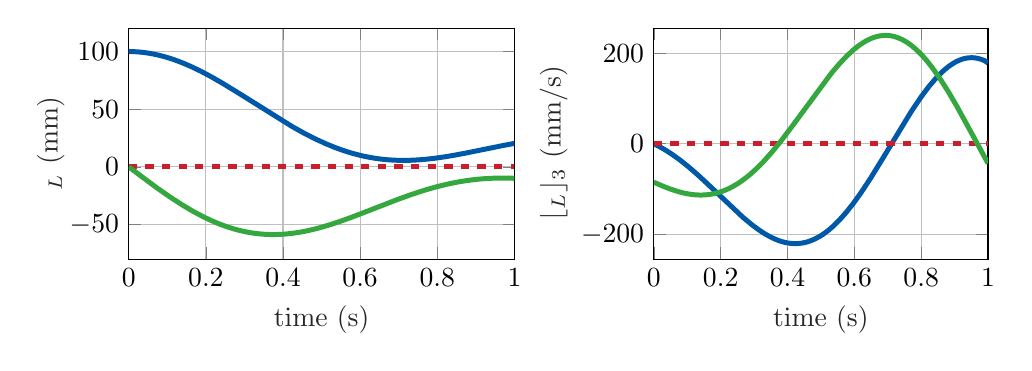
\begin{tikzpicture}

\begin{axis}[%
width=0.404\textwidth,
height=0.242\textwidth,
at={(0\textwidth,0\textwidth)},
scale only axis,
xmin=0,
xmax=1,
xlabel style={font=\color{white!15!black}},
xlabel={time (s)},
ymin=-80,
ymax=120,
ylabel style={font=\color{white!15!black}, yshift=-5pt},
ylabel={$ \gammaB_L $ (mm)},
axis background/.style={fill=white},
xmajorgrids,
ymajorgrids
]
\addplot [color=mycolor1, line width=1.8pt, forget plot]
  table[row sep=crcr]{%
0	99.7999999999986\\
0.00223964165734003	99.7973744072979\\
0.00449943757030269	99.7894032385059\\
0.00792751981879292	99.767107765435\\
0.0125714285714338	99.7173004640467\\
0.0184971098265834	99.6210311814633\\
0.0257913247362183	99.452280688556\\
0.0332936979785927	99.2210910832167\\
0.0423216444981875	98.8658806195815\\
0.0530209617755872	98.3369383055835\\
0.0641509433962284	97.6639557908219\\
0.0772200772200762	96.7166959455565\\
0.0909090909090935	95.5467878395046\\
0.106901217861974	93.9568805106074\\
0.123783031988879	92.0281272017212\\
0.143472022955521	89.4714374015077\\
0.164444444444442	86.4101333623327\\
0.18683001531393	82.7938810486975\\
0.213036565977745	78.1602278968701\\
0.243781094527364	72.2715315545542\\
0.282722513088999	64.3063809929585\\
0.424742268041243	34.6940007741157\\
0.456289978678043	28.8516670741767\\
0.48571428571428	23.871796037797\\
0.512415349887135	19.8066564245194\\
0.535796766743644	16.6367309774332\\
0.555294117647065	14.2885395322973\\
0.57553956834532	12.1448265237983\\
0.591240875912405	10.6930865097043\\
0.607407407407408	9.39254512644054\\
0.624060150375939	8.25899429506282\\
0.635443037974682	7.60378300142125\\
0.647058823529406	7.03423289670161\\
0.658914728682177	6.55469252560214\\
0.671018276762396	6.16929840847122\\
0.683377308707122	5.88191113471227\\
0.689655172413794	5.77608373790237\\
0.695999999999998	5.69604441721829\\
0.702412868632706	5.64216535125435\\
0.708894878706204	5.61478685126646\\
0.715447154471548	5.61421450680018\\
0.722070844686655	5.64071621420031\\
0.728767123287668	5.69451908923003\\
0.735537190082638	5.7758062658089\\
0.742382271468145	5.8847135837659\\
0.749303621169915	6.02132616948518\\
0.763380281690146	6.37773285763318\\
0.777777777777771	6.84455691872186\\
0.792507204610956	7.42028289582042\\
0.807580174927111	8.10222526586492\\
0.823008849557525	8.88640182404758\\
0.846846846846844	10.2421105128154\\
0.871559633027516	11.7904200606828\\
0.914826498422713	14.7034263044896\\
0.970491803278691	18.4693803844847\\
1	20.3165545629562\\
};
\addplot [color=mycolor2, dashed, line width=1.8pt, forget plot]
  table[row sep=crcr]{%
0	0\\
1	0\\
};
\addplot [color=mycolor3, line width=1.8pt, forget plot]
  table[row sep=crcr]{%
0	-3.61537644266718e-09\\
0.0713375796178326	-17.7527567284248\\
0.108548168249662	-26.4200000781221\\
0.139800285306706	-33.1589453228339\\
0.166419019316493	-38.4117614769386\\
0.191063174114021	-42.8146338118347\\
0.213036565977745	-46.3297315753307\\
0.234042553191486	-49.3028883796995\\
0.253781512605045	-51.7351240646114\\
0.271944922547334	-53.6535687304242\\
0.288224956063267	-55.1074641079331\\
0.302325581395351	-56.1616626598023\\
0.313974591651544	-56.8884769641568\\
0.325966850828728	-57.5006769173563\\
0.33519553072626	-57.8782397258901\\
0.344632768361585	-58.1807553089183\\
0.354285714285716	-58.4035154552598\\
0.36084452975048	-58.5053548545591\\
0.367504835589941	-58.5681942694681\\
0.37087378640777	-58.5845408731258\\
0.374269005847957	-58.590599517956\\
0.37769080234834	-58.5861909109014\\
0.381139489194496	-58.571136056554\\
0.384615384615387	-58.5452564332206\\
0.391650099403577	-58.4603122857785\\
0.398797595190381	-58.3299470804194\\
0.406060606060606	-58.1527699697726\\
0.417177914110432	-57.7962604946399\\
0.428571428571431	-57.3269294930165\\
0.440251572327043	-56.7405951666252\\
0.452229299363054	-56.0334115463667\\
0.46868250539957	-54.8966784026617\\
0.485714285714288	-53.5325062963644\\
0.503355704697988	-51.9365006858544\\
0.526315789473685	-49.6133068372119\\
0.550351288056206	-46.9300986419265\\
0.580722891566268	-43.2572802692019\\
0.624060150375939	-37.6831067649934\\
0.695999999999998	-28.3676834706202\\
0.728767123287675	-24.4112162828547\\
0.756302521008401	-21.3424247030881\\
0.777777777777779	-19.1493034122343\\
0.799999999999997	-17.0901855500341\\
0.823008849557525	-15.2042364723099\\
0.838805970149252	-14.0630781987289\\
0.854984894259822	-13.0289142111722\\
0.871559633027523	-12.1136848286582\\
0.888544891640869	-11.3289912044061\\
0.905956112852664	-10.6858555921471\\
0.914826498422713	-10.4205913115741\\
0.923809523809524	-10.1944465403014\\
0.932907348242814	-10.0085079561308\\
0.942122186495176	-9.86376804711688\\
0.95145631067961	-9.76111344196095\\
0.960912052117266	-9.70131271469189\\
0.970491803278691	-9.68500369162139\\
0.980198019801982	-9.71268029736685\\
0.990033222591364	-9.78467898662958\\
1	-9.90116481945083\\
};
\end{axis}

\begin{axis}[%
width=0.35\textwidth,
height=0.242\textwidth,
at={(0.55\textwidth,0\textwidth)},
scale only axis,
xmin=0,
xmax=1,
xlabel style={font=\color{white!15!black}},
xlabel={time (s)},
ymin=-255,
ymax=255,
ylabel style={font=\color{white!15!black}, yshift=-2pt},
ylabel={$\lfloor \etaB_L \rfloor_3$ (mm/s)},
axis background/.style={fill=white},
xmajorgrids,
ymajorgrids
]
\addplot [color=mycolor1, line width=1.8pt, forget plot]
  table[row sep=crcr]{%
0	-5.03322894473968e-09\\
0.0173010380622713	-6.50220495361191\\
0.0358422939067964	-14.3948686496833\\
0.055762081784394	-23.9101852620639\\
0.0772200772200904	-35.297915417717\\
0.1020134228188	-49.7946691493567\\
0.130801687763721	-68.160583968584\\
0.166419019316493	-92.5546161263635\\
0.26666666666668	-162.348077306552\\
0.293805309734523	-178.950648064041\\
0.313974591651544	-189.974031478974\\
0.33209647495363	-198.706228867454\\
0.34782608695653	-205.256001077113\\
0.360844529750466	-209.878175746971\\
0.374269005847964	-213.827254496507\\
0.384615384615387	-216.27114612029\\
0.395209580838326	-218.206632761828\\
0.402414486921543	-219.183899865081\\
0.40973630831644	-219.888164780211\\
0.417177914110425	-220.29924144634\\
0.420944558521569	-220.388325155136\\
0.424742268041228	-220.396212237696\\
0.428571428571416	-220.320179200681\\
0.432432432432421	-220.15746161557\\
0.436325678496871	-219.905255785567\\
0.4442105263158	-219.120979710955\\
0.452229299363069	-217.944212726521\\
0.460385438972168	-216.351332000494\\
0.468682505399556	-214.318325348871\\
0.481400437636751	-210.390407883886\\
0.494456762749451	-205.3351325721\\
0.507865168539325	-199.070676986792\\
0.521640091116183	-191.517360981173\\
0.535796766743658	-182.599579632315\\
0.555294117647065	-168.468401954006\\
0.575539568345334	-151.652697767758\\
0.596577017114925	-132.059585351932\\
0.618453865336647	-109.658142704518\\
0.64705882352942	-77.7974783343005\\
0.683377308707122	-34.4105554254838\\
0.770538243626049	71.379609065326\\
0.800000000000011	103.623297293933\\
0.82300884955751	126.278762663014\\
0.846846846846859	146.810719886305\\
0.863221884498472	158.911390922616\\
0.879999999999995	169.4328859242\\
0.89719626168224	178.094573094596\\
0.905956112852664	181.637421317512\\
0.914826498422713	184.605752163697\\
0.923809523809524	186.962407397604\\
0.932907348242821	188.670244303364\\
0.942122186495169	189.692354493835\\
0.951456310679617	189.992307751626\\
0.960912052117266	189.534422304558\\
0.970491803278691	188.284062879113\\
0.980198019801975	186.207967787265\\
0.990033222591364	183.274606180161\\
1	178.254201447696\\
};
\addplot [color=mycolor2, dashed, line width=1.8pt, forget plot]
  table[row sep=crcr]{%
0	0\\
1	0\\
};
\addplot [color=mycolor3, line width=1.8pt, forget plot]
  table[row sep=crcr]{%
0	-85.0473803587339\\
0.00223964165732582	-85.6158257265569\\
0.0282685512367493	-93.9745343566354\\
0.0489596083231447	-99.8692813302412\\
0.0655737704917954	-103.986025188536\\
0.0802069857697347	-107.075842816235\\
0.0924702774108255	-109.230655828393\\
0.103633916554514	-110.815531789786\\
0.113543091655259	-111.899935113828\\
0.122052704576987	-112.575419257088\\
0.129032258064512	-112.945239904325\\
0.134370579915128	-113.1123265999\\
0.137980085348516	-113.167094032888\\
0.139800285306706	-113.176630107849\\
0.141630901287556	-113.173872976656\\
0.143472022955535	-113.158519828933\\
0.147186147186147	-113.088786901727\\
0.15094339622641	-112.964898631011\\
0.15666178623718	-112.671762328688\\
0.162481536189063	-112.241611387335\\
0.170403587443957	-111.43807150471\\
0.17851739788199	-110.349211758237\\
0.188940092165893	-108.547163238602\\
0.199687987519496	-106.204281487471\\
0.210776545166397	-103.262328044361\\
0.224555735056555	-98.8535168541872\\
0.238879736408563	-93.3782523458157\\
0.25378151260503	-86.7157831311057\\
0.269296740994861	-78.7404165295425\\
0.28822495606326	-67.605560082891\\
0.308108108108115	-54.3087274508757\\
0.329020332717192	-38.6632488696587\\
0.354285714285709	-17.7087082305252\\
0.38113948919451	6.65961839144884\\
0.417177914110425	41.8824215281318\\
0.531034482758628	155.4887375113\\
0.555294117647065	176.545560445766\\
0.575539568345334	192.374387721705\\
0.596577017114925	206.808308760275\\
0.612903225806463	216.404103229858\\
0.62972292191435	224.672732502005\\
0.641221374045813	229.316042501543\\
0.652956298200507	233.166210099722\\
0.664935064935065	236.135529841472\\
0.671018276762396	237.26166879576\\
0.677165354330697	238.13345171144\\
0.683377308707122	238.73922529072\\
0.689655172413779	239.067251513411\\
0.695999999999998	239.10573840527\\
0.702412868632706	238.842874076787\\
0.70889487870619	238.266864236387\\
0.715447154471548	237.365973386964\\
0.722070844686641	236.128569919031\\
0.728767123287668	234.543175316821\\
0.742382271468131	230.283589889617\\
0.756302521008394	224.500600761065\\
0.770538243626049	217.113959654515\\
0.785100286532952	208.052212548924\\
0.800000000000011	197.255482171009\\
0.815249266862168	184.678627371514\\
0.830860534124639	170.294793777077\\
0.854984894259815	145.327990555536\\
0.879999999999995	116.392775121539\\
0.905956112852664	83.7617660698862\\
0.951456310679617	22.5887905891359\\
1	-43.2445730182744\\
};
\end{axis}
\end{tikzpicture}%
  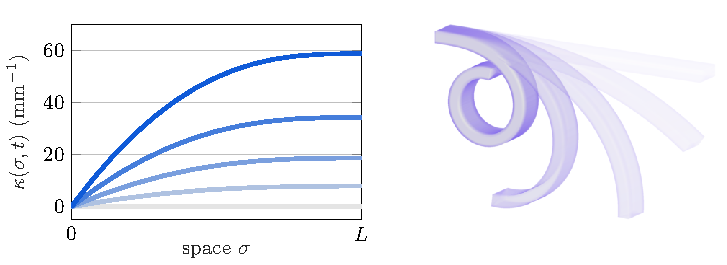
\includegraphics{./pdf/thesis-figure-5-2-1.pdf}  \\[0.15em]
  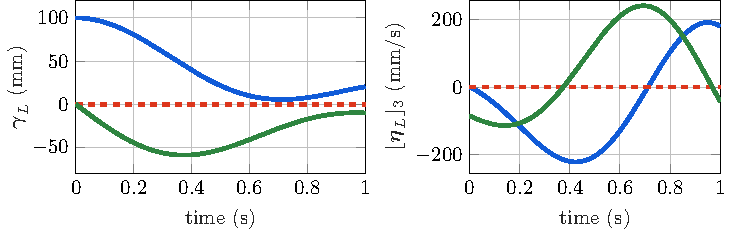
\includegraphics{./pdf/thesis-figure-5-2-2.pdf}  
  \caption{Spatio-temporal evolution of the cantilever beam obtained by solving the exact continuum forward kinematics described in \eqref{eq:C3:cont_kin_pde}. The figure shows the forward kinematic solutions of the end-effector position $\gammaB_L:=\gammaB(L)$ and its linear velocities $\lfloor \etaB_L \rfloor_3:=\lfloor \etaB(L) \rfloor_3$, where the following color coding is used $\{x,y,z\} = \{\ldatanum{Matlab1}{},\ldatanum{Matlab2}{},\ldatanum{Matlab3}{}\}$.}
  \vspace{-0.2cm}
  \label{fig:C3:EX1:cantilever_FK_example}
\end{figure}

Then, substitution of $\sB_i$, $\vB_i$ and $\aB_i$ into \eqref{eq:C3:cont_kin_pde} leads to an ordinary differential equation that depends exclusively on $\sigma$. The forward kinematics can then be solved for the spatial horizon $\Xs = [0,L]$ using an explicit integration routine (fourth order Runge Kutta method), which produces $\gB$, $\etaB$ and $\dot{\etaB}$. We repeat this process until the full forward kinematics is recovered for all $t \in \Ts$. The results for the Euler-Bernoulli cantilever beam are shown in Figure \ref{fig:C3:EX1:cantilever_FK_example}. Figure \ref{fig:C3:EX1:cantilever_FK_example} shows for $\kappa(\sigma,t)$ evolves over space and time, and how they relate to the continuum deformations. It also shows the position $\gammaB_L$ and the linear velocities $\lfloor \etaB \rfloor_3$ of the end-effector. Note that this approach can easily deal with non-constant curvature situations, in contrast to the approach discussed in Chapter \ref{chap:PCC}. Namely, Chapter \ref{chap:PCC} subdivided the domain $\Xs$ into small PCC segments leading to notorious discontinuities at the interfaces (see Figure \ref{fig:C4:basis_example}).

\end{example}


% %
% Since we assume the $\mat{g}$ to be everywhere differentiable, we can derive a PDE for the continuous forward kinematics of the soft robot \cite{Boyer2021,Renda2020}:
% %
% \begin{equation}
% \dfrac{\p \vec{\eta}}{\p \sigma} = -\textbf{ad}_{\vec{\xi}} \vec{\eta} + \dot{\vec{\xi}},
% \label{eq:pde_kin}
% \end{equation}
% %
% where $\ad_{(\cdot)}$ denotes the adjoint action on the Lie algebra (full derivation in Appendix A). Drawing an analogy to rigid robotics, the expression in \eqref{eq:pde_kin} may be seen as the forward velocity kinematics for a serial chain robot manipulator with infinitely many links.

%%%%%%%%%%%%%%%%%%%%%%%%%%%%%%%%%%%%%%%%%%%%%%%%%%
\subsection{Finite-dimensional projection}
The problem is, however, that the exponential coordinates of the geometric strain vector belong (in theory) to an infinite set of real-valued functions. Similar to many continuum mechanics problems, the state dimension for such multi-variable coordinate representation are of infinite dimensional nature. To solve this, we must project our solution space onto a finite dimensional subset that is countable and therefore computable in this setting. In the finite element method, the solution presents itself by dividing the continuum into a finite set of elements. Here we follow an approach similar to Chirikjian et al. \cite{Chirikjian1991,Chirikjian1992} that proposed to express the spatial deformations of slender (semi-rigid) continuum robots by finite set of basis functions called \textit{spatial modes}. This idea also finds application is disturbance rejection for structural vibration of semi-rigid flexible manipulators whose modeling strategies are identical the Euler-Bernoulli assumptions. Here though we introduce a modal approximation to find a suitable finite-dimensional approximation of the strain twist $\vec{\xi}(\sigma,t)$ for all points along the material domain $\Xs$. To do so, we assume the following: %
\begin{asm}
\vspace{1mm}
Assuming the strain field has a separable spatio-temporal nature, any entry of the strain vector field $\vec{\xi} = \left( \xi_1, \xi_2, ..., \xi_6 \right)^\top$ can be written as an infinite expansion of the following form:
%
\begin{equation}
\xi_i(\sigma,t) = \sum_{n=1}^\infty \theta_{n}(\sigma)q_{i,n}(t) + \xi^\circ_{i}(\sigma) \quad i\in\{1,\hdots,6\},
\label{eq:infinite_expans}
\end{equation}
%
where $\{\theta_{n}\}^\infty_{n=1}$ is a set of (orthogonal) basis functions $\theta_{n}: \Xs \to \R$ together with modal coefficients $q_{i,n}: \Ts \to \R$, and an intrinsic time-invariant strain $\xi^\circ_{i}: \Xs \to \R$. The basis functions $\theta_{n}(\cdot)$ and the modal coefficients $q_n(\cdot)$ are both smooth functions.
\end{asm}

\begin{asm}
Given infinite expansion \eqref{eq:infinite_expans}, the $k$-th order truncation for any entry of the strain field, defined as
%
\begin{equation}
[\xi_i]_k(\sigma,t) := \sum_{n=1}^k \theta_n(\sigma)q_{i,n}(t) + \xi^\circ_{i}(\sigma) \quad i\in\{1,\hdots,6\},
\end{equation}
%
converges uniformly on $\Xs$ and $\Ts$ as the index $k \to \infty$. Moreover, we assume that uniform convergence holds for its partial derivatives $\tfrac{\p}{\p t} [\vec{\xi}]_k$ and $\tfrac{\p}{\p \sigma} [\vec{\xi}]_k$.
\end{asm}

\noindent Accordingly, we can rewrite the $k$-th order truncation of the complete strain field as a linear matrix operation as follows
%
\begin{align}
[\vec{\xi}]_k  & = \left(\vec{I}_6  \otimes \begin{bmatrix} \theta_1 & \hdots & \theta_k \end{bmatrix} \right) \vec{q} + \vec{\xi}^\circ,  \notag \\[0.5em]
& =
\begingroup % keep the change local
\setlength\arraycolsep{2.5pt}
\underbrace{\begin{pmatrix}
\theta_1 & \hdots & \theta_k & \hdots & 0 & \cdots&  0 \\
\vdots & \ddots & \vdots & \ddots & \vdots & \vdots & \vdots \\
0 & \cdots&  0 & \hdots & \theta_1 & \hdots & \theta_k\end{pmatrix}}_{{\mat{\Theta}(\sigma)}}
\endgroup
\underbrace{\begin{pmatrix} q_{1,1} \\ \vdots \\ q_{6,k}\end{pmatrix}}_{\vec{q}(t)} + \vec{\xi}^\circ,
\label{eq:trunc_2}
%\vspace{-4mm}
\end{align}
%
where $\mat{\Theta} \in \R^{6 \times 6k}$ is a sparse matrix-valued function whose columns are mutually orthonormal, the operator $\otimes$ denotes the Kronecker product, and the vector $\vec{q} \in \R^{6k}$ the collection of all time-varying modal coefficients related to the columns of $\mat{\Theta}$. Although a wide variety of bases are possible (see for instance \cite{Boyer2021,DellaSantina2020}), we have chosen a modified Legendre polynomial set:
%
\begin{figure}[!t]
  \vspace{-1mm}
    %\centering
    %\ifx\printFigures\undefined
    %\else$$
    \hspace{0.7mm}
    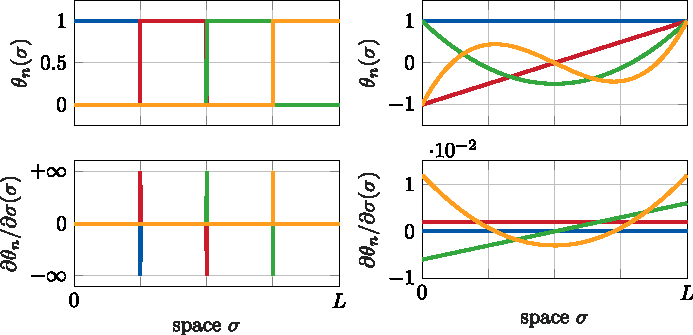
\includegraphics[width=.95\textwidth]{./pdf/thesis-figure-5-3.pdf}
    %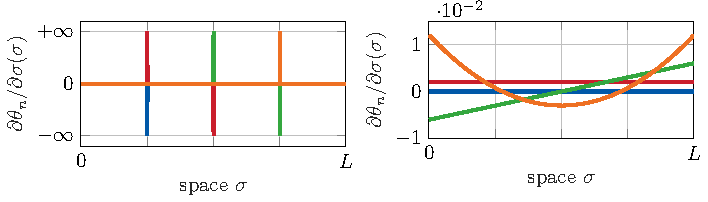
\includegraphics[width=\textwidth]{./pdf/thesis-figure-5-3-2.pdf}
    %% This file was created by matlab2tikz.
%
\definecolor{mycolor1}{rgb}{0.00000,0.34510,0.65882}%
\definecolor{mycolor2}{rgb}{0.79216,0.11765,0.17255}%
\definecolor{mycolor3}{rgb}{0.20392,0.65490,0.24706}%
\definecolor{mycolor4}{rgb}{0.93333,0.43922,0.13725}%
%
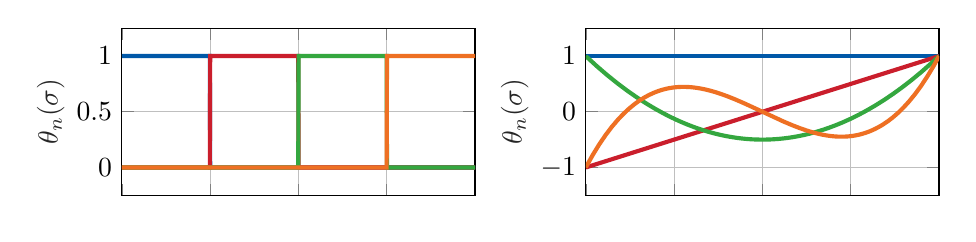
\begin{tikzpicture}

\begin{axis}[%
width=0.37\textwidth,
height=0.175\textwidth,
at={(0\textwidth,0\textwidth)},
scale only axis,
xmin=0,
xmax=1,
xtick={0,0.25,0.5,0.75,1},
xticklabels={{},{},{},{},{}},
ymin=-0.25,
ymax=1.25,
ylabel style={font=\color{white!15!black}},
ylabel={$\theta_n(\sigma)$},
axis background/.style={fill=white},
title style={font=\bfseries},
% title={$(a)$},
xmajorgrids,
ymajorgrids,
ylabel style={yshift=-2.5pt}
]
\addplot [color=mycolor1, line width=1.5pt, forget plot]
  table[row sep=crcr]{%
0	1\\
0.249249249249249	1\\
0.25025025025025	0\\
1	0\\
};
\addplot [color=mycolor2, line width=1.5pt, forget plot]
  table[row sep=crcr]{%
0	0\\
0.249249249249249	0\\
0.25025025025025	1\\
0.499499499499499	1\\
0.500500500500501	0\\
1	0\\
};
\addplot [color=mycolor3, line width=1.5pt, forget plot]
  table[row sep=crcr]{%
0	0\\
0.499499499499499	0\\
0.500500500500501	1\\
0.74974974974975	1\\
0.750750750750751	0\\
1	0\\
};
\addplot [color=mycolor4, line width=1.5pt, forget plot]
  table[row sep=crcr]{%
0	0\\
0.74974974974975	0\\
0.750750750750751	1\\
1	1\\
};
\end{axis}

\begin{axis}[%
width=0.37\textwidth,
height=0.175\textwidth,
at={(0.486\textwidth,0\textwidth)},
scale only axis,
xmin=0,
xmax=1,
xtick={0,0.25,0.5,0.75,1},
xticklabels={{},{},{},{},{}},
ymin=-1.5,
ymax=1.5,
ylabel style={font=\color{white!15!black}},
ylabel={$\theta_n(\sigma)$},
axis background/.style={fill=white},
title style={font=\bfseries},
%title={$(b)$},
xmajorgrids,
ymajorgrids,
ylabel style={yshift=-2.5pt}
]
\addplot [color=mycolor1, line width=1.5pt, forget plot]
  table[row sep=crcr]{%
0	1\\
1	1\\
};
\addplot [color=mycolor2, line width=1.5pt, forget plot]
  table[row sep=crcr]{%
0	-1\\
1	1\\
};
\addplot [color=mycolor3, line width=1.5pt, forget plot]
  table[row sep=crcr]{%
0	1\\
0.0310310310310311	0.819591363134907\\
0.0610610610610611	0.656004352701049\\
0.0900900900900901	0.508156805454103\\
0.118118118118118	0.375002630257885\\
0.145145145145145	0.255531808084361\\
0.171171171171171	0.148770392013635\\
0.196196196196196	0.0537805072339606\\
0.22022022022022	-0.0303396489582677\\
0.243243243243243	-0.10445580715851\\
0.265265265265265	-0.169397625854082\\
0.286286286286286	-0.225958691424157\\
0.307307307307307	-0.277217157097037\\
0.327327327327327	-0.321104888672456\\
0.346346346346346	-0.358343328313298\\
0.364364364364364	-0.389617846074302\\
0.381381381381381	-0.415577739902064\\
0.397397397397397	-0.436836235635034\\
0.413413413413414	-0.455016578139701\\
0.428428428428429	-0.469265060856652\\
0.442442442442442	-0.480122765408051\\
0.456456456456456	-0.488623758894029\\
0.469469469469469	-0.494407320233146\\
0.482482482482482	-0.498158819480141\\
0.495495495495496	-0.499878256635014\\
0.507507507507508	-0.499661823986148\\
0.519519519519519	-0.497713930146363\\
0.532532532532533	-0.493649805962118\\
0.545545545545546	-0.487553619685752\\
0.558558558558559	-0.479425371317263\\
0.572572572572573	-0.468399330261192\\
0.586586586586587	-0.455016578139701\\
0.601601601601602	-0.438062687311937\\
0.617617617617618	-0.416996576155735\\
0.633633633633634	-0.392852311771231\\
0.650650650650651	-0.363826288751214\\
0.668668668668669	-0.329305281257233\\
0.687687687687688	-0.288639991342694\\
0.707707707707708	-0.241145048952857\\
0.727727727727728	-0.188840492143795\\
0.748748748748749	-0.128744359975591\\
0.770770770770771	-0.0600991381772165\\
0.793793793793794	0.0178887596305013\\
0.817817817817818	0.106048991934878\\
0.842842842842843	0.205247289331373\\
0.868868868868869	0.316385454523592\\
0.894894894894895	0.435651868084301\\
0.921921921921922	0.56810864918973\\
0.94994994994995	0.714729744759775\\
0.978978978978979	0.876525173822471\\
1	1\\
};
\addplot [color=mycolor4, line width=1.5pt, forget plot]
  table[row sep=crcr]{%
0	-1\\
0.0190190190190189	-0.782485871940692\\
0.0380380380380381	-0.585849574761409\\
0.0560560560560561	-0.418072891875022\\
0.0740740740740742	-0.267591322461007\\
0.0910910910910911	-0.14071778835241\\
0.107107107107107	-0.0342981766697772\\
0.123123123123123	0.0600275897464979\\
0.138138138138138	0.137912741624562\\
0.153153153153153	0.206008053341874\\
0.167167167167167	0.26108942025359\\
0.18018018018018	0.305205863277448\\
0.193193193193193	0.342823368979655\\
0.205205205205205	0.372007618203764\\
0.216216216216216	0.394270823050955\\
0.227227227227227	0.412405233898399\\
0.237237237237237	0.425443028180901\\
0.246246246246246	0.434472266818126\\
0.255255255255255	0.441030078586554\\
0.264264264264264	0.445204206451941\\
0.272272272272272	0.446984357566612\\
0.28028028028028	0.447012056580584\\
0.288288288288288	0.445348928183114\\
0.297297297297297	0.441533571555485\\
0.306306306306306	0.435743998198344\\
0.316316316316316	0.427102419377978\\
0.327327327327327	0.41505036134801\\
0.339339339339339	0.399043011303921\\
0.352352352352352	0.378569076902044\\
0.367367367367367	0.351233983600084\\
0.383383383383384	0.318131447265587\\
0.401401401401401	0.276624908126279\\
0.422422422422422	0.223395060218871\\
0.447447447447447	0.154754895576799\\
0.481481481481481	0.0554285423969925\\
0.55955955955956	-0.174453117166602\\
0.585585585585586	-0.244218652545899\\
0.606606606606607	-0.295588205146412\\
0.625625625625626	-0.337224912399687\\
0.641641641641642	-0.368091627977139\\
0.656656656656657	-0.393078784510256\\
0.66966966966967	-0.411320689517806\\
0.681681681681682	-0.42510521776274\\
0.692692692692693	-0.434982658462395\\
0.702702702702703	-0.441533571555485\\
0.711711711711712	-0.445348928183114\\
0.720720720720721	-0.447102325115474\\
0.728728728728729	-0.446858939689107\\
0.736736736736737	-0.444855399075886\\
0.744744744744745	-0.441030078586554\\
0.753753753753754	-0.434472266818126\\
0.762762762762763	-0.425443028180901\\
0.771771771771772	-0.413854619709123\\
0.781781781781782	-0.3978703949716\\
0.792792792792793	-0.376369795653945\\
0.803803803803804	-0.350609329511154\\
0.815815815815816	-0.317460398130658\\
0.827827827827828	-0.278843238464521\\
0.840840840840841	-0.230596015489016\\
0.854854854854855	-0.170884130911225\\
0.868868868868869	-0.10280934270289\\
0.883883883883884	-0.020216582116821\\
0.898898898898899	0.0727618041999487\\
0.914914914914915	0.183843708779055\\
0.931931931931932	0.315873496183937\\
0.948948948948949	0.462912686785208\\
0.966966966966967	0.635618141204809\\
0.984984984984985	0.826515637191178\\
1	1\\
};
\end{axis}
\end{tikzpicture}%
    %% This file was created by matlab2tikz.
%
\definecolor{mycolor1}{rgb}{0.00000,0.34510,0.65882}%
\definecolor{mycolor2}{rgb}{0.79216,0.11765,0.17255}%
\definecolor{mycolor3}{rgb}{0.20392,0.65490,0.24706}%
\definecolor{mycolor4}{rgb}{0.93333,0.43922,0.13725}%
%
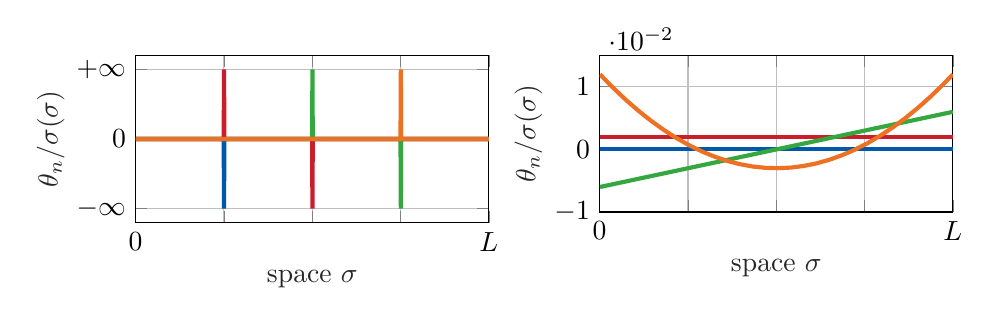
\begin{tikzpicture}

\begin{axis}[%
width=0.37\textwidth,
height=0.175\textwidth,
at={(0\textwidth,0\textwidth)},
scale only axis,
xmin=0,
xmax=1,
xtick={0,0.25,0.5,0.75,1},
xticklabels={{0},{},{},{},{$L$}},
ytick={-1,0,1},
yticklabels={{$-\infty$},0,{$+\infty$}},
xlabel style={font=\color{white!15!black}},
xlabel={space $\sigma$},
ymin=-1.2,
ymax=1.2,
ylabel style={font=\color{white!15!black}},
ylabel={$\p \theta_n/\p \sigma (\sigma)$},
axis background/.style={fill=white},
xmajorgrids,
ymajorgrids,
ylabel style={yshift=-2.5pt}
]
\addplot [color=mycolor1, line width=1.5pt, forget plot]
  table[row sep=crcr]{%
0.00100100100100109	0\\
0.249249249249249	0\\
0.25025025025025	-1\\
0.251251251251251	0\\
1	0\\
};
\addplot [color=mycolor2, line width=1.5pt, forget plot]
  table[row sep=crcr]{%
0.00100100100100109	0\\
0.249249249249249	0\\
0.25025025025025	1\\
0.251251251251251	0\\
0.499499499499499	0\\
0.500500500500501	-1\\
0.501501501501502	0\\
1	0\\
};
\addplot [color=mycolor3, line width=1.5pt, forget plot]
  table[row sep=crcr]{%
0.00100100100100109	0\\
0.499499499499499	0\\
0.500500500500501	1\\
0.501501501501502	0\\
0.74974974974975	0\\
0.750750750750751	-1\\
0.751751751751752	0\\
1	0\\
};
\addplot [color=mycolor4, line width=1.5pt, forget plot]
  table[row sep=crcr]{%
0.00100100100100109	0\\
0.74974974974975	0\\
0.750750750750751	1\\
0.751751751751752	0\\
1	0\\
};
\end{axis}

\begin{axis}[%
width=0.37\textwidth,
height=0.164\textwidth,
at={(0.486\textwidth,0.011\textwidth)},
scale only axis,
xmin=0,
xmax=1,
xtick={0,0.25,0.5,0.75,1},
xticklabels={{0},{},{},{},{$L$}},
xlabel style={font=\color{white!15!black}},
xlabel={space $\sigma$},
ymin=-0.01,
ymax=0.015,
ylabel style={font=\color{white!15!black}},
ylabel={$\p \theta_n/\p \sigma(\sigma)$},
axis background/.style={fill=white},
xmajorgrids,
ymajorgrids,
ylabel style={yshift=-2.5pt}
]
\addplot [color=mycolor1, line width=1.5pt, forget plot]
  table[row sep=crcr]{%
0.00100100100100109	0\\
1	0\\
};
\addplot [color=mycolor2, line width=1.5pt, forget plot]
  table[row sep=crcr]{%
0.00100100100100109	0.00200200200200196\\
1	0.00200200200200196\\
};
\addplot [color=mycolor3, line width=1.5pt, forget plot]
  table[row sep=crcr]{%
0.00100100100100109	-0.00599999398798179\\
1	0.00599999398798179\\
};
\addplot [color=mycolor4, line width=1.5pt, forget plot]
  table[row sep=crcr]{%
0.00100100100100109	0.0119819719820118\\
0.037037037037037	0.00989780573368138\\
0.0730730730730731	0.00796962698002934\\
0.109109109109109	0.00619743572105302\\
0.145145145145145	0.00458123195675597\\
0.181181181181181	0.00312101568713552\\
0.217217217217217	0.00181678691219256\\
0.253253253253253	0.000668545631927309\\
0.289289289289289	-0.000323708153660229\\
0.325325325325325	-0.00115997444457028\\
0.361361361361361	-0.00184025324080306\\
0.397397397397397	-0.0023645445423579\\
0.433433433433434	-0.00273284834923548\\
0.469469469469469	-0.00294516466143557\\
0.505505505505506	-0.00300149347895817\\
0.541541541541542	-0.00290183480180284\\
0.577577577577578	-0.00264618862997024\\
0.613613613613614	-0.00223455496346037\\
0.64964964964965	-0.00166693380227234\\
0.685685685685686	-0.000943325146407048\\
0.721721721721722	-6.37289958642651e-05\\
0.757757757757758	0.000971854649356008\\
0.793793793793794	0.00216342578925377\\
0.82982982982983	0.00351098442382924\\
0.865865865865866	0.00501453055308221\\
0.901901901901902	0.00667406417701244\\
0.937937937937938	0.00848958529562016\\
0.973973973973974	0.0104610939089056\\
1	0.0119819719820118\\
};
\end{axis}
\end{tikzpicture}%
    %\fi
    %\vspace{-3mm}
    \caption{Example plot of the Constant-Strain parametrization in Chapter 3 (left), and the new strain parametrization \eqref{eq:C3:chebyshev} using Chebyshev polynomials (right). The ordering of the strain basis is as follows $\{\theta_1,...,\theta_4\} = \{\ldata{Matlab1},\ldata{Matlab2},\ldata{Matlab3},\ldata{Matlab4}\}$. Notice that the
    spatialdiscontinuities in the PCC model induces spikes that directly violate the compatibility equation in \eqref{eq:C3:compatibility}.}
    \label{fig:C4:basis_example}
  \end{figure}
  %
\begin{equation}
\theta_n(\sigma) = \dfrac{2}{2^{n}(n-1)!} \dfrac{d^{n-1}}{d\sigma^{n-1}}\left[\left( \dfrac{2\sigma}{L}-1 \right)^2 -1 \right]^{n-1}
\label{eq:C3:chebyshev}
\end{equation}
%
\noindent with $n \in \mathbb{Z}_{>0}$ the polynomial degree A comparison between the proposed basis and previous method in Chapter \ref{chap:PCC} is shown in Figure \ref{fig:C4:basis_example}.
Important to note is that the previous PCC condition discussed introduces discontinuities in space that violate the compatibility equation in \eqref{eq:C3:compatibility}. 
Also note now that the inner product between elements of the set of modified Legendre functions $\{\theta_n\}_{n = 1}^k$ satisfies $\inner{\theta_i}{\theta_j}_{\Xs} := \int_\Xs{\theta_i}{\theta_j} d\sigma = 0$ for $i \neq j$, and $1$ otherwise. An alternative option could be constructing the set of basis functions through the so-called '\textit{snapshot decomposition method}' \cite{Astrid2008,Duriez2013,Largilliere2015}.

% \begin{rmk}
% The idea of joint parameterization by investigating the relation between material and structural topology of the soft robot is explored in Chapter 5.
% \end{rmk}

\subsection{Reduced-order kinematics}
Given the finite-dimensional truncation in \eqref{eq:trunc_2}, we can now find an expression for the finite-dimensional forward kinematics in terms of the generalized coordinates $\vec{q}$ and its velocities components $\dot{\vec{q}}$.

First, let us regard the configuration of the soft robot $\mat{g} \in \SE{3}$. Recall that the spatial evolution of the curve is described by $\p \mat{g}/\p\sigma = \mat{g} \vec{\xi}^\wedge$, see \eqref{eq:C3:xi}. Given the initial condition $\mat{g}(0,\cdot) = \mat{g}_0$, an approximation of the continuously deformable soft robot can be obtained by partial integration over the spatial domain:
%
\vspace{-2mm}
\begin{equation}
[\mat{g}]_k(\sigma,\vec{q}) = \mat{g}_0 \exp_{\SE{3}}\left(\int_0^\sigma [\hat{\vec{\xi}}]_k(s,\vec{q}) \; ds \right).
\end{equation}
%
The computation of the mapping $\exp_{\SE{3}}$ is given in Appendix \ref{app:C3:liegroup}. Note that the expression above nothing more than the reconstruction of the curve by integration of its tangent space along its spatial parameter $\sigma$. Next, lets regard the velocity kinematics $\vec{\eta}(\sigma,t)$ for any point $\sigma$ on the backbone curve. Using the differential property of the adjoint action $\mat{\ad}_{\vec{\xi}} = -\p /\p \sigma [\Ad_{g^{-1}}] \Ad_{g}$ \cite{Murray1994}, we can rewrite the
continuum forward kinematics in \eqref{eq:C3:pde_kin} as
%
\begin{equation}
\frac{\p \vec{\eta}}{\p \sigma } = \frac{\p }{\p \sigma }\left(\mat{\Ad}_{\mat{g}^{-1}}\right) \mat{\Ad}_{\mat{g}} \vec{\eta} + \dot{\vec{\xi}}. \label{eq:eta_adg}
\end{equation}
%
Now, given the initial condition $\vec{\eta}(0,t) = \vec{0}_6$ and the approximations $[\vec{\xi}]_k$ and $[\mat{g}]_k$, we can find an approximation to the velocity twist $\vec{\eta}$ by partial integration over space:
%
\begin{equation}
[\vec{\eta}]_k(\sigma,\vec{q},\dot{\vec{q}}) = \Ad_{[\mat{g}]_k(\sigma,\q)}\inv \int_0^\sigma \Ad_{[\mat{g}]_k(s,\q)} \mat{\Theta}(s) \dot{\vec{q}} \; ds \,. \label{eq:C3:eta_analytic}
\end{equation}
%
Note from \eqref{eq:C3:eta_analytic} that the joint velocity exhibits a linear relationship with the velocity twist. This attribute is typical of rigid robotics, \eg, see \cite{Murray1994,Spong2006}. As such, it is possible to extract $\dot{\q}$ out of the integrand which naturally gives rise to a linear matrix transformation called the \textit{"geometric manipulator Jacobian"}. The geometric Jacobian matrix $[\mat{J}]_k \in \R^{6\times 6k}$ is defined by 
%
\begin{equation}
[\mat{J}]_k:= \Ad_{[\mat{g}]_k(\sigma,\q)}\inv \int_0^\sigma \Ad_{[\mat{g}]_k(s,\q)} \mat{\Theta}(s) \; ds, \label{eq:C3:jacobian_analytic}
\end{equation}
%
such that $[\etaB]_k = [\JB]_k \dot{\q}$. The geometric Jacobian plays an important role in obtaining the Lagrangian form of the reduced-order dynamic model. Finally, to express the acceleration twist, we take the time-derivative of \eqref{eq:C3:eta_analytic} leading to
%
\begin{align}
[\dot{\vec{\eta}}]_k & = [\mat{J}]_k\ddot{\vec{q}} + \dot{[\mat{J}]}_k\dot{\vec{q}}, \notag \\
& = [\mat{J}]_k\ddot{\vec{q}} + \Ad_{[\mat{g}]_k}\inv \int_0^\sigma \Ad_{[\mat{g}]_k(s,\q)} \ad_{[\vec{\eta}]_k(s,\q,\dq)} \mat{\Theta}(s) \; ds \,\dot{\q} \label{eq:C3:deta_analytic},
\end{align}
%
which gives rise to the analytic expression of the time-derivative of the geometric Jacobian $\dot{[\mat{J}]}_k$.
Although the expression for the $\dot{\JB}$ is compact, its derivation is fairly involved. We therefore refer the reader to Appendix \ref{app:C3:jacobian} on its derivation. 
\subsection{Reduced-order dynamics using Newton-Euler}
Here, we detail the dynamics of the Cosserat beam. A majority of the dynamic framework presented here is adopted from Boyer et al. \cite{Boyer2021}; yet we introduce some modification to allow a pH-structure. Other works that adopt a similar approach include \cite{Renda2018,Renda2020,Till2019,Garofalo2013}. First, let us consider an infinitesimal slice of continuum body that is perpendicular to the backbone curve. The kinetic momenta of this infinitesimal slice is then given by $\vec{\mu}(\sigma,t) := \MT \vec{\eta}(\sigma,t)$ in which $\MT \in \cose{3} \times \seg{3} \cong \R^{6\times 6}$ denotes the symmetric inertia tensor.
%
\begin{rmk}
  For some soft robots, the inertia tensor $\MT$ may have an explicit dependency on space or time (or both). A common phenomena in soft robotics that innately lead to such dependencies include for instance the \textit{ballooning effect} of soft pneumatic networks. During actuation, matter expands outwards radially, changing the cross-sectional geometry and thus its inertial properties. That said, the inertial changes due to ballooning is negligibly small. Besides, ballooning is often an undesired phenomena that is reduced by appropriate structural design such as internal ribs, or bellow-like geometries. Nevertheless, examples where inertial changes cannot be neglected include the class of growing or morphing soft robots \cite{Hawkes2017,Joachimczak2014Jul,Joachimczak2015}, self-healing soft robots \cite{Terryn2021Jul,Roels2020Dec}, origami soft robot manipulators \cite{Li2022Nov,Jiang2016Dec,Wu2021Sep}. Pressure-driven soft robots actuated by near incompressible fluids like water also suffer from these inertial changing effects. But, these robots are scarce and purposefully design for aquatic environments which is outside the scope of this work. For many soft robots, air or gas is preferred over liquids. 
For sake of simplicity, we limit ourselves to a diagonal invariant inertia tensor: 
%
\begin{equation*}
\MT(\sigma,t) \simeq \begin{pmatrix} \rho_0 \ten{J}  & \vec{0}_{3\times3}  \\[0.35em]
  \vec{0}_{3\times3} & \rho_0\, A_0\mat{I}_3 \end{pmatrix} \succ 0,
\end{equation*}
%
in which the (cross-sectional average) density is $\rho_0 > 0$, the cross-sectional area of the soft robot $A_0>0$, and the second moment of area $\mat{\mathcal{J}} \in \coso{3} \times \sog{3} \cong \R^{3\times 3}$.
We emphasize here that considering an invariant cross-sectional inertia tensor is not an overly conservative assumption. It still holds true for a large class of soft manipulators, and it has limited effects on the generality of our modeling framework. \end{rmk}
%
\noindent Using the expression of the kinetic momenta $\muB(\sigma,t)$ of the infinitesimal rigid body in free-motion, we can write the equation of motion for a particular slice at $\sigma$ using the Newton-Euler equations:
%
\begin{equation}
\frac{\p }{\p t} (\Ad_{\gB}^{-\top} \vec{\mu}) = \Ad_{g}^{-\top}\ten{F},\label{eq:C3:newton_euler}
\end{equation}
%
where again $\Ad_{(\cdot)}$ stands for the adjoint action, and $\ten{F} = \ten{F}_c  + \ten{F}_u - \ten{F}_\textrm{b} - \ten{F}_{\textrm{mat}}$ the resultant wrench that is composed of the constraint wrench $\ten{F}_c$, the input wrench $\ten{F}_u$, and the potential wrenches due to body accelerations and hyper- and visco-elasticity, $\ten{F}_\textrm{b}$ and $ \ten{F}_{\textrm{mat}}$, respectively. Further evaluation of \eqref{eq:C3:newton_euler} leads to
%
\begin{equation}
\MT\dot{\vec{\eta}} - \ad_{\vec{\eta}}^\top \MT \vec{\eta} = \ten{F},
\label{eq:C3:newton-euler-2}
\end{equation}
%
where we used the fact that $\tfrac{\p}{\p t}{\Ad}_{\vec{g}} \inv = -\ad_{\vec{\eta}} {\Ad}_{\vec{g} \inv}$. Before continuing, we introduce a slight modification to the relation above. Using the fact that $\ad_{\vec{\eta}} \vec{\eta} = \vec{0}_6$, we can introduce the vector
$\ten{M} \ad_{\vec{\eta}} \vec{\eta}$ to \eqref{eq:C3:newton-euler-2} without affecting the dynamics. The importance of this modification originates from the preservation of passivity in the Lagrangian model, which is an important property in stability theorems for robotics. By substitution of the null vector, the equation of motion becomes
%
\begin{equation}
  \MT \dot{\vec{\eta}} + \left(\MT \ad_{\vec{\eta}}  - \ad_{\vec{\eta}} ^\top \MT \right) \vec{\eta} = \FT,
  \label{eq:C3:newton-euler-3}
\end{equation}
%
which is nothing more than the Newton-Euler equation for rigid-body motion on $\R^3$. To introduce the (reduced-order) Cosserat kinematics and make the expression symmetric, we substitute \eqref{eq:C3:eta_analytic} and \eqref{eq:C3:deta_analytic} into \eqref{eq:C3:newton-euler-3} and pre-multiply by $[\JB]_k^\top$:
%
\begin{align}
  [\vec{J}]_k^\top \left( \MT [\mat{J}]_k \ddot{\vec{q}} + \MT [\dJB]_k\dot{\vec{q}} + \CT_{[\vec{\eta}]_k }\dot{\vec{q}}\right) = [\mat{J}]_k^\top \left(\FT_u - \FT\grav -  \ten{F}_{\textrm{mat}} \right),
  \label{eq:C3:projected_NE_jacobian}
\end{align}
%
where $\CT_{(\cdot)} = -\CT_{(\cdot)} ^\top :=  \MT \ad_{(\cdot)}  - \ad_{(\cdot)} ^\top \MT$ is a skew-symmetric matrix. It is important to note that by pre-multiplication of the transpose Jacobian, we have eliminated the constraint wrenches, \ie, $[\JB]_k^\top \FT_c = \vec{0}_n$ \cite{Murray1994}. Finally, the finite-dimensional dynamics of the deformable soft robot is found by spatial integration of \eqref{eq:C3:projected_NE_jacobian} over the material domain $\Xs$. The overall dynamics can be written in the familiar Euler-Lagrangian (EL) form as follows
%
\begin{equation}
  \mat{M}(\vec{q})\ddot{\vec{q}} + \mat{C}(\vec{q},\dot{\vec{q}})\dot{\vec{q}} + \vec{f}\!\grav(\vec{q}) + \vec{f}_{\textrm{mat}}(\vec{q},\dot{\vec{q}}) = \vec{\tau}(\vec{q},\uB)
  \label{eq:C3:dyn_model_lag}
\end{equation}
%
with the system matrices:
%
\begin{align}
 \MB(\q) & = \int_\Xs [\mat{J}]_k^\top \ten{M} [\mat{J}]_k \; d \sigma, \label{eq:C3:lag_M} \\
 \mat{C}(\q,\dq) & = \int_\Xs [\JB]_k^\top \!\left(\ten{M} [\dJB]_k + \ten{C}_{{[\vec{\eta}]}_k}[\mat{J}]_k \right) \; d \sigma, \label{eq:C3:lag_C} \\
\vec{f}\!\grav(\q) & = \int_\Xs [\JB]_k^\top \ten{F}_\textrm{b} \; d \sigma, \\
\vec{f}_{\textrm{mat}}(\q,\dq) & = \int_\Xs [\JB]_k^\top  \ten{F}_{\textrm{mat}} \; d \sigma =: \mat{K}\vec{q} + \mat{D}\dot{\vec{q}},
\label{eq:C3:lag_G} \\
\vec{\tau}(\q,\uB) & = \int_\Xs [\mat{J}]_k^\top \ten{F}_u \; d\sigma =: \mat{G}(\q) \vec{u}, \label{eq:C3:lag_tau}
\end{align}
%
\noindent where $\mat{M}$ is the generalized inertia matrix, $\mat{C}$ the  Centripetal-Coriolis matrix, $\fB\!\grav$ a vector of generalized potential forces with $\ten{F}_\textrm{b} = -\Ad_{[\gB]_k}^\top \ten{M} \vec{a}_b$ the external wrench acting on the body due to body-frame accelerations $\vec{a}_b$ (like gravity), and $\ten{F}_\textrm{mat}$ a vector of visco-elastic material forces imposed by the stiffness matrix $\mat{K} \succ 0$ and damping matrix $\vec{D} \succ 0$. The derivation for these constant matrices is shown in Appendix \ref{app:C3:linearmaterialmatrices}, where it is shown that stiffness and damping matrix are computed through spatial integration similar to standard finite element methods:
%
\begin{align}
\mat{K} = \int_\Xs \mat{\Theta}^\top \!\mat{\mathcal{K}}\, \mat{\Theta} \; d\sigma, \label{eq:C3:stiff_mat}\\
\mat{D} = \int_\Xs \mat{\Theta}^\top \!\mat{\mathcal{D}}\, \mat{\Theta} \; d\sigma, \label{eq:C3:damp_mat}
\end{align}
%
where $\mat{\mathcal{K}} \in \cose{3} \times \seg{3}$ and $\mat{\mathcal{D}} \in  \cose{3} \times \seg{3}$ are the stiffness and damping tensor, respectively.
The vector $\vec{Gu}$ represents the distributed forces $\nB_\textrm{u}(\sigma,t)$ and moments $\mB_\textrm{u}(\sigma,t)$ generated by various kinds of the internal actuators (\eg, tendons or pneumatics). We will later detail the derivation of $\GB(\q)$ in this chapter as it depends highly on the geometrical placement of the soft actuators. If $\rank(\GB) < \dim(\q)$, the system \eqref{eq:C3:dyn_model_lag} is said to be underactuated. Within the context of soft robotics, whose infinite-dimensional configuration space cannot be matched by a finite number of actuators, these systems are often intrinsically under-actuated. 

To compute the Lagrangian matrices \eqref{eq:C3:lag_M}-\eqref{eq:C3:damp_mat}, that all involve a spatial integration over $\Xs = [0,L]$, we rewrite these integrations into one global matrix differential equation and solve it efficiently using a Matrix-Differential solver proposed in Chapter \ref{chap:PCC}. As such, these system matrices are not computed exactly but approximated with sufficient precision. The numerical precision depends on the stepsize of the discretized spatial domain $\Xs$. 
\begin{asm}
\label{lem:C3:1}
The inertia matrix $\mat{M}(\vec{q})$ is a symmetric, positive definite, symmetric. and is uniformly bounded such that there exists positive constants $\lambda^{-} \le \lambda^{+}$ such that  $\lambda^{-} \mat{I}_{n} \preceq \mat{M}(\vec{q}) \preceq \lambda^{+} \mat{I}_{n} < \infty$.
\end{asm}

The uniform boundedness of the inertia matrix $\MB(\q)$ is a well-known property for rigid manipulators composed of purely rotational joints. According to Spong et al. \cite{Spong2006} the inertia matrix in this case is composed solely of $\cos(\cdot)$ and $\sin(\cdot)$ terms, and thus it is bounded for all $\q \in \mathcal{Q}$. The physical interpretation is that the mass and moment of inertia of the robot must be finite and positive for all configurations. This does not always hold true for instance for robots with prismatic joints. Yet, bounds can be imposed on the configuration space $\q \in \mathcal{Q}$ that enable boundedness, see Ghorbel et al. \cite{Ghorbel1998Dec}. In Della Santina et al. \cite{DellaSantina2020a}, it was shown that $\MB(\q) = \MB^\top(\q) \succeq 0$ for soft manipulators restricted to variable planar curvatures. The property holds for the infinite dimensional case where $k \to \infty$. 

\begin{lem}
\label{lem:C3:passive}
Given the inertia matrix $\mat{M}(\vec{q})$ and the Coriolis matrix
$\mat{C}(\vec{q},\dot{\vec{q}})$ as described by \eqref{eq:C3:lag_M} and \eqref{eq:C3:lag_C}, respectively, it can be shown that the matrix $\dot{\mat{M}} - 2\mat{C}$ is skew-symmetric.
\end{lem}

\begin{proof}
To show $\dot{\mat{M}} - 2\mat{C}$ is skew-symmetric, we start by computing the time-derivative of the inertia matrix. For sake of clarity, we abbreviate the Jacobian matrices $[\mat{J}]_k = \mat{J}$ and $[\dJB]_k = \dJB$. Through chain differentiation, we find
%
\begin{equation}
\dot{\mat{M}} = \int_\Xs \left(\dJB^\top \ten{M} \mat{J} + \mat{J}^\top \ten{M} \dJB 
\right)\; d \sigma,
\end{equation}
%
Then, calculating $\dot{\mat{M}} - 2\mat{C}$ leads to
%
\begin{align}
\dot{\mat{M}} - 2\mat{C} & = \int_\Xs \dJB^\top \left( \ten{M} \mat{J} - \mat{J}^\top \ten{M} \dJB - 2\mat{J}^\top \!\ten{C} \, \mat{J} \right) \; d\sigma.
\end{align}
%
Since the matrix $\mat{J}^\top \ten{C} \mat{J}$ is skew-symmetric, the remainder of the proof is to show that the matrix $\mat{S} = \dJB^\top \ten{M} \mat{J} - \mat{J}^\top \ten{M} \dJB$ also satisfies skew-symmetry. Since the inertia tensor is symmetric $\ten{M} = \ten{M}^\top
$, we can easily show this holds true:
%
\begin{align}
\mat{S} & = \dJB^\top \MT^\top \mat{J} - \mat{J}^\top \MT^\top \dJB, \notag \\
 & = -\left(\dJB^\top \ten{M}^\top \mat{J} - \mat{J}^\top \ten{M} \dJB \right)^\top = -\mat{S}^\top.
\end{align}
%
Therefore, the matrix $\dot{\mat{M}(\vec{q})} - 2\mat{C}(\vec{q},\dot{\vec{q}})$ is skew-symmetric for all $\vec{q},\dot{\vec{q}} \in \R^n$
\end{proof}

In literature, Lemma \ref{lem:C3:passive} is often referred to as the passivity condition \cite{Spong2006,Ortega1998,Murray1994}. It implies that, in the absence of external dissipation, the total energy of the system (\ie, the Hamiltonian) is conserved.
It is also worth mentioning that this condition does not necessarily hold true for any representation of the Coriolis matrix only for particular computations of the Coriolis matrix $\mat{C}(\vec{q},\vec{\dot{q}})$ (\eg, through the Christoffel symbols).

\subsection{Tendon and fluidic actuation}
Up to now, we have not discussed the derivation of the actuation mapping $\GB(\q)$. The matrix namely depends on $(i)$ the type of actuation, and $(ii)$ how actuation fields are distributed along the backbone curve of the soft robot manipulator. Earlier, we introduced the notion of a distributed forces $\nB_\textrm{u}$ and distributed moments $\mB_\textrm{u}$ acting on the curve $\gB$, which are collocated into a control wrench $\FT_{\textrm{u}}$. Now, assuming that a general soft manipulator system is either actuated using a set of fluidic chambers or a set of tendons, the control wrench related this network of $m$ number of soft actuators can be represented in the form \cite{Renda2020,Boyer2021}:
%
\begin{equation}
\FT_{\textrm{u}}(\sigma,\uB) = \sum_{i = 1}^m \begin{pmatrix}
\rB_i^\times(\sigma) \tB_i(\sigma) \\[0.25em] \tB_i (\sigma)
\end{pmatrix} u_i =: \ThetaB_{\textrm{u}}(\sigma) \uB,
\label{eq:C3:controlwrenchfield}
\end{equation}
%
where $\rB_i: \Xs \to \R^3$ is the radial distance between the actuator center-line and the backbone curve $\gammaB$, and $\tB_i: \Xs \times \mathcal{Q} \to \R^3$ the tangent vector along the actuator center-line expressed that deforms with the continuum body prescribed by $[\gB]_k(\sigma,\q)$, $\ThetaB_\textrm{u} \in \R^{6 \times m}$ a shape function matrix related to the spatial distribution of the soft actuators, and $u_i(t)$ a time-varying scalar related to the activation amplitude of the $i$-th soft actuator. Generally speaking, for tendon actuation $u_i = -\max\{0,\lambda_i\}$ with $\lambda_i$ the cable tension and for pneumatic actuation we have $u_i = A_i p_i$ with $A_i > 0$ an effective pressure surface and $p_i$ the applied pressure. Following \eqref{eq:C3:controlwrenchfield}, the generalized joint torques can then be computed by projecting the distributed control wrench onto the configuration space using the geometric Jacobian matrix. Then, $\GB(\q)$ is computed by integrating generalized distributed joint forces over $\Xs$:
%
\begin{equation}
\tauB(\q,\uB) = \int_{\Xs} \JB^\top(\q,\sigma) \ThetaB_{\textrm{u}}(\sigma)\; d\sigma \,\uB =: \GB(\q) \uB.
\end{equation}
%
Similar to the other Lagrangian matrices, the actuation mapping is included into the matrix differential solver to allow fast and efficient computation of \eqref{eq:C3:dyn_model_lag}.

\subsection{Port-Hamiltonian formulation}
In this section, the Lagrangian model in \eqref{eq:C3:dyn_model_lag} is rewritten in port-Hamiltonian form. To this end, we define the generalized momenta $\vec{p} := \mat{M} \dot{\vec{q}}$. Then, the (reduced-order) Hamiltonian is given by $\mathcal{H}(\vec{q},\vec{p}) := \Kf(\vec{q},\vec{p}) + \Uf(\vec{q})$ with $\Kf = \frac{1}{2} \vec{p}^\top \mat{M}\inv \vec{p}$ and $\Uf(\vec{q})$ the kinetic and potential energy, respectively.

Given the system's Hamiltonian $\mathcal{H}$, it can be shown that generalized velocities can be written in terms of partial derivatives of the Hamiltonian function
%
\begin{equation}
\dot{\vec{q}} = \nabla_{\vec{p}} \Hm \quad \Longrightarrow  \quad \nabla_{\vec{p}} \Hm := \left(\frac{\p \Hm}{\p \pB} \right)^\top= \mat{M}\inv \vec{p}.
\label{eq:C3:state_diff}
\end{equation}
%
where we denote $\nabla_{\xB}(\cdot) := \p (\cdot)^\top/\p \xB$ as the gradient w.r.t. a vector field $\xB$. Note that $\mat{M}^{-1}$ is always exists due to the positive definiteness condition in Lemma \ref{lem:C3:1}. Similarly, we seek a differential description that relates the time evolution of $\vec{p}$ to a state-derivative of the Hamiltonian function. Applying the chain rule of differentiation to the generalized momenta:
%
\begin{align}
\dot{\vec{p}} & = \dot{\mat{M}}\dot{\vec{q}} + \mat{M}\ddot{\vec{q}},\notag \\
& = \left(\dot{\mat{M}} - \mat{C} - \mat{D} \right) \mat{M}\inv \vec{p} - \vec{Kq} - \vec{f}\!\grav + \vec{Gu}
\label{eq:C3:momenta_diff1},
\end{align}
%
Taking the partial derivative of the Hamiltonian $\Hm$ w.r.t. the generalized coordinates $\vec{q}$, we find
 %
\begin{align}
\nabla_{\vec{q}} \Hm & = \frac{1}{2} \,\nabla_{\!\q} \left[ \dot{\vec{q}}^\top \mat{M}(\vec{q}) \dot{\vec{q}} \right] + \nabla_{\!\vec{q}}\, \mathcal{U}.
\label{eq:C3:ham_momenta_diff}
\end{align}
%
To relate \eqref{eq:C3:momenta_diff1} and \eqref{eq:C3:ham_momenta_diff}, we explores some structural properties in the Lagrangian model. To be more specific, we exploit the skew-symmetry condition as detailed in Lemma \ref{lem:C3:passive}. According to the Spong et al. (2006, \cite{Spong2006}), if the matrix $\dot{\mat{M}} - 2\mat{C}$ satisfies the
skew-symmetry in Lemma \ref{lem:C3:passive}, it can be shown that
%
\begin{equation}
\left( \dot{\mat{M}} - 2\mat{C} \right) \dot{\vec{q}} =  -\nabla_{\vec{q}} \left[ \dot{\vec{q}}^\top \mat{M}(\vec{q}) \dot{\vec{q}} \right] - \dot{\mat{M}}\dot{\vec{q}}. \label{eq:C3:skew_mat_equal}
\end{equation}
%
Finally, by combining \eqref{eq:C3:state_diff}, \eqref{eq:C3:momenta_diff1}, \eqref{eq:C3:ham_momenta_diff}, and \eqref{eq:C3:skew_mat_equal}, we can show that the Lagrangian model in \eqref{eq:C3:dyn_model_lag} can be equivalently rewritten as a standard port-Hamiltonian (pH) system:
\begin{align}
\Sigma_{\textrm{beam}}: 
\begin{cases}
\dot{\vec{q}} \;=\; \nabla_{\vec{p}} \Hm, \\[0.25em]
\dot{\vec{p}} \;=\; -\nabla_{\vec{q}} \Hm - \mat{D}\nabla_{\vec{p}} \Hm + \vec{Gu}.
\end{cases}
\label{eq:C3:model_ph}
\end{align}
%
The advantage of the port-Hamiltonian system $\Sigma_\textrm{beam}$ over the standard EL structure in \eqref{eq:C3:dyn_model_lag}, and as also seen in Chapter \ref{chap:PCC}, is the general applicability to different physical domains and the common formalism with energy-based control, which we will explore further in the next section. 

%By collocating the state variable into a state vector $\x = (\q^\top, \pB^\top)^\top$, we may write the system into an equivalent form: $\dx = \left(\JT - \RT \right)\grad{\x}\!\Hm(\x) + \BT(\x)\uB$, where $\JT = -\JT^\top$ a skew-symmetric matrix, $\RT \succeq 0$ a positive semi-definite dissipation matrix. 
